\documentclass[a4paper]{report}
\usepackage[utf8]{inputenc}
\usepackage[portuguese]{babel}
\usepackage{hyperref}
\usepackage{a4wide}
\hypersetup{pdftitle={Trabalho 1},
pdfauthor={João Teixeira, José Ferreira, Maria Silva, Miguel Solino},
colorlinks=true,
urlcolor=blue,
linkcolor=black}
\usepackage{subcaption}
\usepackage[cache=false]{minted}
\usepackage{listings}
\usepackage{booktabs}
\usepackage{multirow}
\usepackage{appendix}
\usepackage{tikz}
\usepackage{authblk}
\usepackage{bashful}
\usepackage{verbatim}
\usepackage{amsmath}
\usetikzlibrary{positioning,automata,decorations.markings}

\begin{document}

\title{Fase 1\\ 
\large Grupo Nº 8}
\author{João Teixeira (A85504) \and José Ferreira (A83683) \and Maria Silva (A83840) \and Miguel Solino (A86435)}

\date{\today}

\begin{center}
    \begin{minipage}{0.75\linewidth}
        \centering
        
\includegraphics[width=0.4\textwidth]{images/eng.jpeg}\par\vspace{1cm}
        \vspace{1cm}
        \href{https://www.uminho.pt/PT}
        {\color{black}{\scshape\LARGE Universidade do Minho}} \par
        \vspace{1cm}
        \href{https://www.di.uminho.pt/}
        {\color{black}{\scshape\Large Departamento de Informática}} \par
        \maketitle
    \end{minipage}
\end{center}

\begin{figure}[H]
\centering
\begin{subfigure}{.5\textwidth}
  \centering
  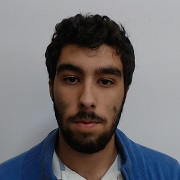
\includegraphics[width=.25\linewidth]{images/A85504.jpeg}
    \caption{João Teixeira (A85504)}
\end{subfigure}%
\begin{subfigure}{.5\textwidth}
  \centering
  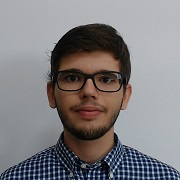
\includegraphics[width=.25\linewidth]{images/A83683.jpeg}
    \caption{José Ferreira (A83683)}
\end{subfigure}
\begin{subfigure}{.5\textwidth}
  \centering
  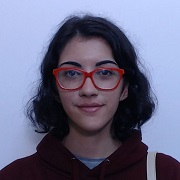
\includegraphics[width=.25\linewidth]{images/A83840.jpeg}
    \caption{Maria Silva (A83840)}
\end{subfigure}%
\begin{subfigure}{.5\textwidth}
  \centering
  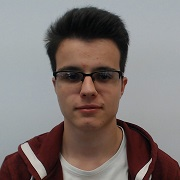
\includegraphics[width=.25\linewidth]{images/A86435.jpeg}
    \caption{Miguel Solino (A86435)}
\end{subfigure}
\end{figure}

\tableofcontents

\pagebreak

\chapter{Introdução}

Este relatório tem como objetivo apresentar a fase inicial do projeto da Unidade
Curricular de Desenvolvimento de Sistemas de Software.\\
Ao longo deste relatório apresentamos as considerações tidas em conta pelo grupo
ao longo da elaboração e formulação dos vário modelos e diagramas propostos:
\begin{enumerate}
    \item Modelo de Domínio, modelo conceptual que contém os
        comportamentos e dados;
    \item Use Cases, apresentar os atores do sistema e as suas tarefas;
    \item Diagrama de Use Cases;
    \item Especificações dos mesmos.
\end{enumerate}
Por fim irá ser apresentado um \textit{mockup} do produto final.

\chapter{Modelo de Domínio}

O sistema a implementar deve suportar a gestão de media e utilização da mesma
numa residência onde esteja instalado.\\
Neste capítulo são apresentados os requisitos do problema e uma proposta de 
Modelo de Domínio.

\section{Descrição do Modelo de Domínio}

O problema em questão consiste em desenvolver um sistema de gestão e streaming
de media.\\
Após analisar o enunciado disponibilizado, concluímos que era necessário a
existência de vários conceitos a incluir na modelação do problema: Utilizador,
Media (música e vídeo), Biblioteca de media, Caracterização (do media que for
adicionada ao sistema por um utilizador), Download/Upload de media, Conta,
Conexões (de amizades entre utilizadores, ou seja, uma lista de Amigos).\\
Com isto, foram definidas as relações entre os conceitos referidos em cima:
\begin{itemize}
    \item cada Utilizador só pode ter uma conta, só pode fazer download do
        media que fez upload e só pode classificar o media e bibliotecas
        que lhe pertencem;
    \item cada media/biblioteca de media pode ter uma ou mais classificações;
    \item cada conta tem só um email, nome e password associados;
    \item conta não é obrigatório para utilizar o sistema mas fica limitado 
        a só usufruir de media;
\end{itemize}
Os utilizadores não devem ter a permissão de criar contas, logo para um
utilizador ter uma conta precisa que outro com permissões de administrador crie
uma conta sem password para mais tarde o utilizador da conta em questão a
defina.

\section{Modelo de Domínio}

\begin{figure}[H]
	\centering 
    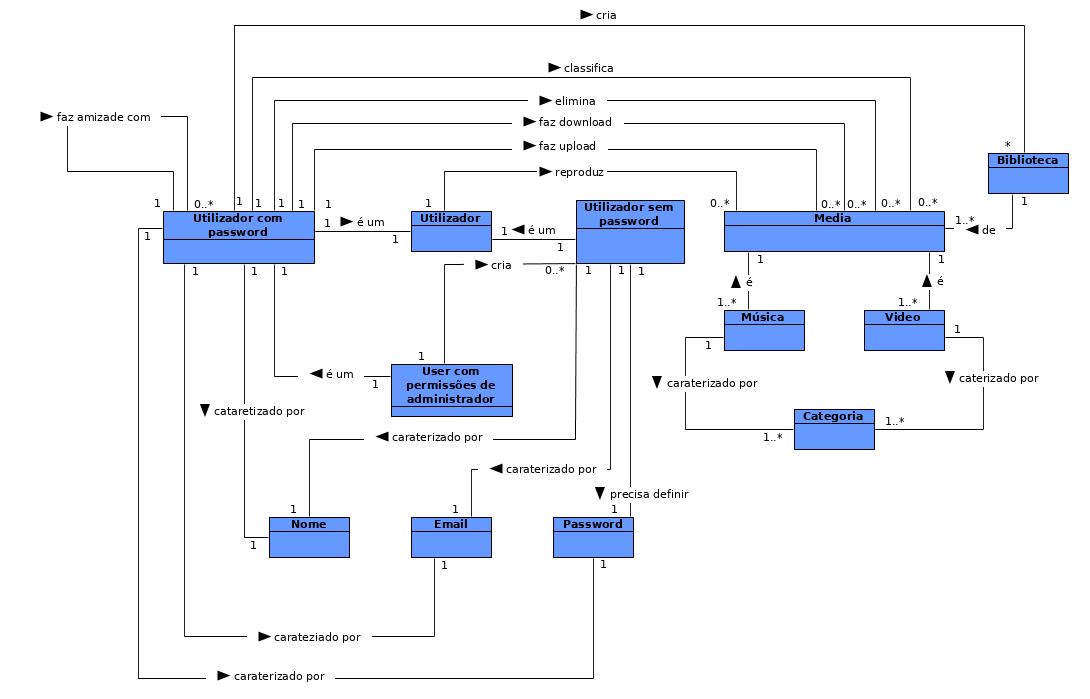
\includegraphics[width=\textwidth]{images/Dominio.png}  
    \caption{Modelo de Domínio}
\end{figure}


\chapter{Use Cases}

O Diagrama de Use Cases representa os atores do sistema e as tarefas de cada um
deles. No nosso caso existem 4 atores:
\begin{itemize}
    \item \textbf{Convidado}: Todos os outros referidos abaixo são atores deste
        tipo. Logo, a este ator estará relacionado as ações que todos podem
        fazer;
    \item \textbf{Utilizador}: Tem acesso à totalidade de ações que um
        user sem permissões de administrador pode ter;
    \item \textbf{Administrador}: A diferença deste 
        utilizador para os restantes é que este é o único que pode criar uma
        conta e assim ser o responsável pela existência dos restantes.
\end{itemize}

\begin{figure}[H]
	\centering 
    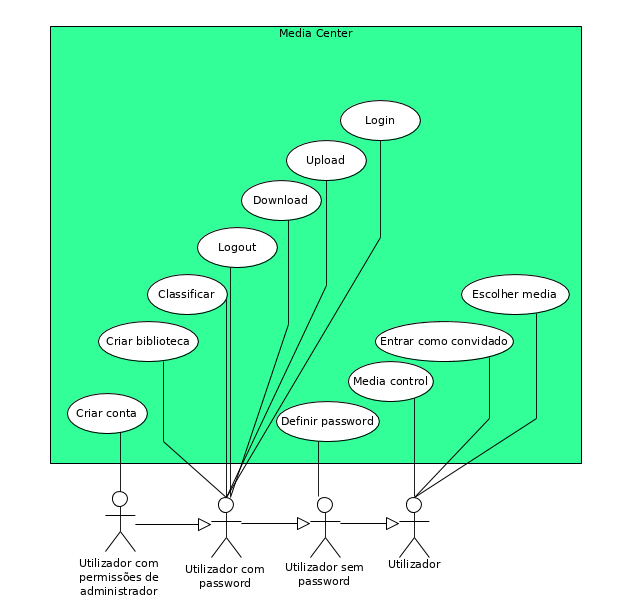
\includegraphics[width=\textwidth]{images/UseCases.png}  
    \caption{Diagrama de Use Cases}
\end{figure}

\pagebreak

\section{Especificações dos Use Cases}

Nesta parte optamos por ordenar os use cases por permissões, ou seja, começamos
por apresentar os de um utilizador normal, seguido de um utilizador sem
password, utilizador com password e utilizador com permissões de administrador.

\subsection{Entrar como convidado}

\begin{figure}[H]
	\centering 
    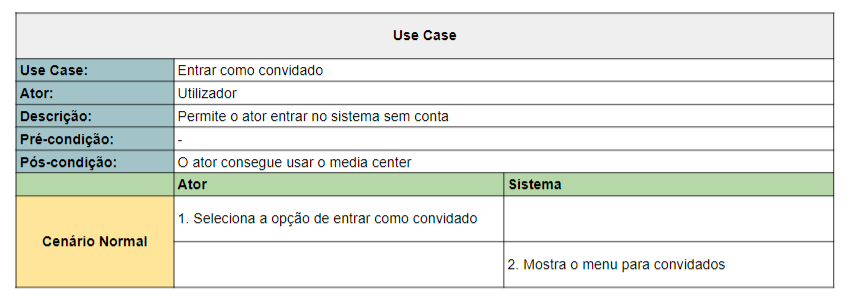
\includegraphics[width=\textwidth]{images/Entrar_como_convidado.png}  
    \caption{Especificação do \emph{Use Case} Entrar como convidado}
\end{figure}

\subsection{Reproduzir Conteúdo}

\begin{figure}[H]
	\centering 
    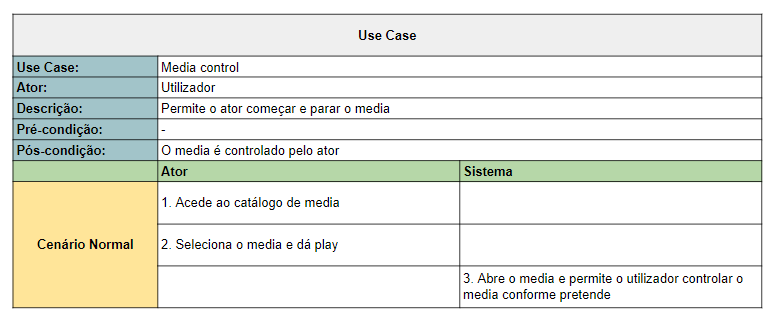
\includegraphics[width=\textwidth]{images/Media_Control.png}  
    \caption{Especificação do \emph{Use Case} Reproduzir Conteúdo}
\end{figure}

\subsection{Editar Utilizador}

\begin{figure}[H]
	\centering 
    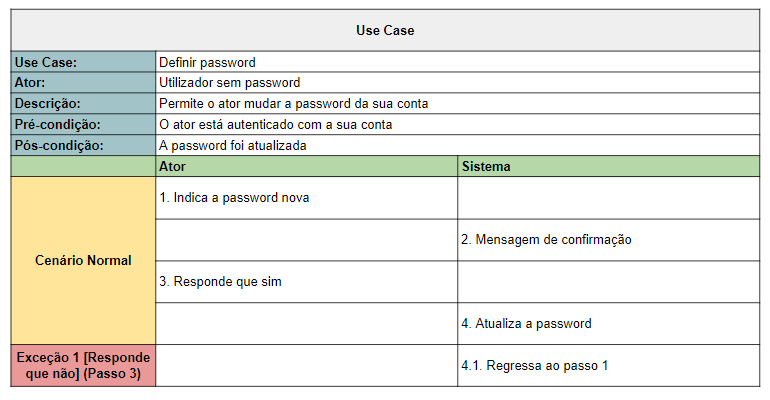
\includegraphics[width=\textwidth]{images/Definir_Password.png}  
    \caption{Especificação do \emph{Use Case} Editar Utilizador}
\end{figure}

\subsection{Login}

\begin{figure}[H]
	\centering 
    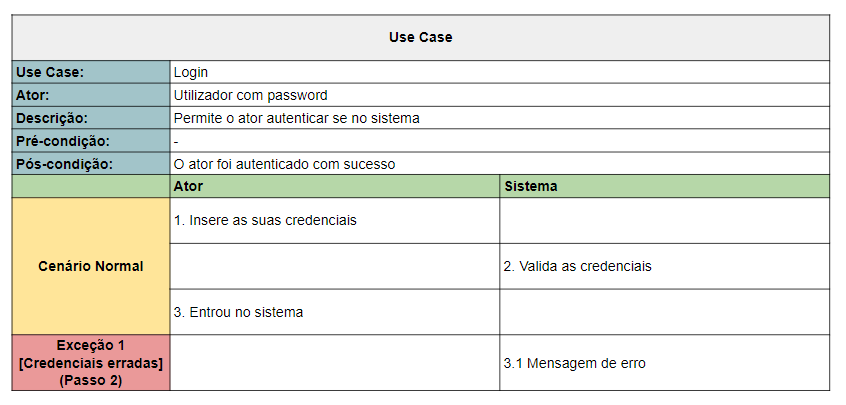
\includegraphics[width=\textwidth]{images/Login.png}  
	\caption{Especificação do \emph{Use Case} Login}
\end{figure}

\subsection{Logout}

\begin{figure}[H]
	\centering 
    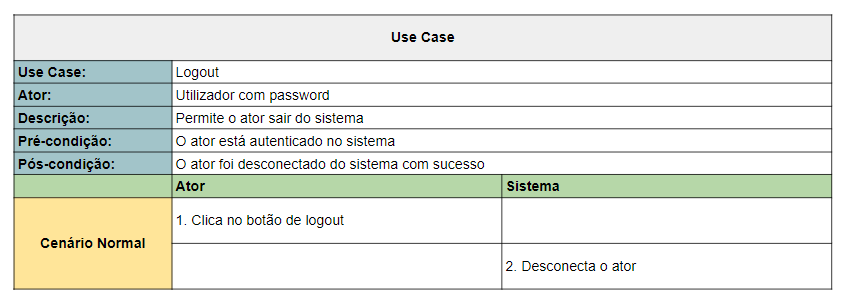
\includegraphics[width=\textwidth]{images/Logout.png}  
    \caption{Especificação do \emph{Use Case} Logout}
\end{figure}

\subsection{Download}

\begin{figure}[H]
	\centering 
    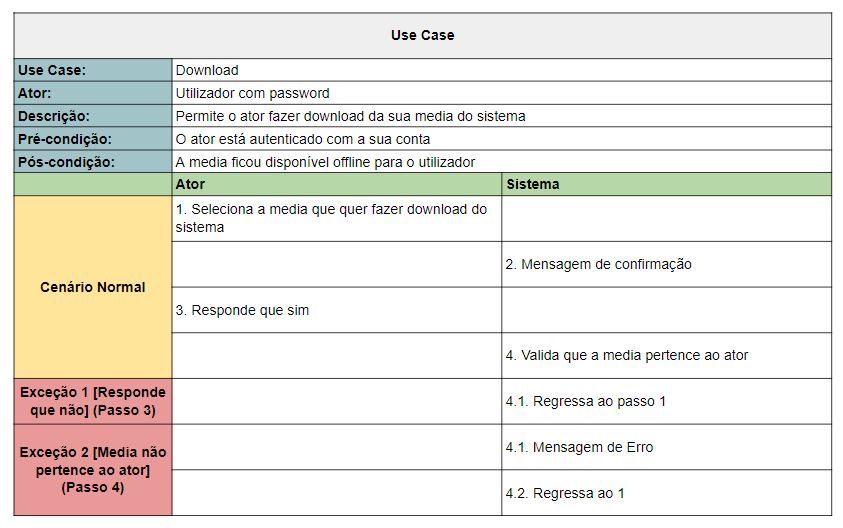
\includegraphics[width=\textwidth]{images/Download.png}  
    \caption{Especificação do \emph{Use Case} Download}
\end{figure}

\subsection{Upload}

\begin{figure}[H]
	\centering 
    \includegraphics[width=\textwidth]{images/upload.png}  
    \caption{especificação do \emph{use case} upload}
\end{figure}

\subsection{Remover Conteúdo}

\begin{figure}[H]
	\centering 
    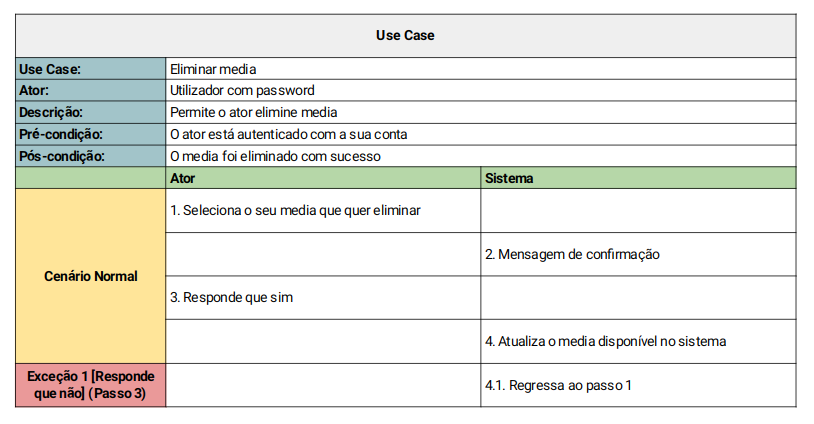
\includegraphics[width=\textwidth]{images/Eliminar_media.png}  
    \caption{especificação do \emph{use case} Remover Conteúdo}
\end{figure}

\subsection{Alterar Categoria}

\begin{figure}[H]
	\centering 
    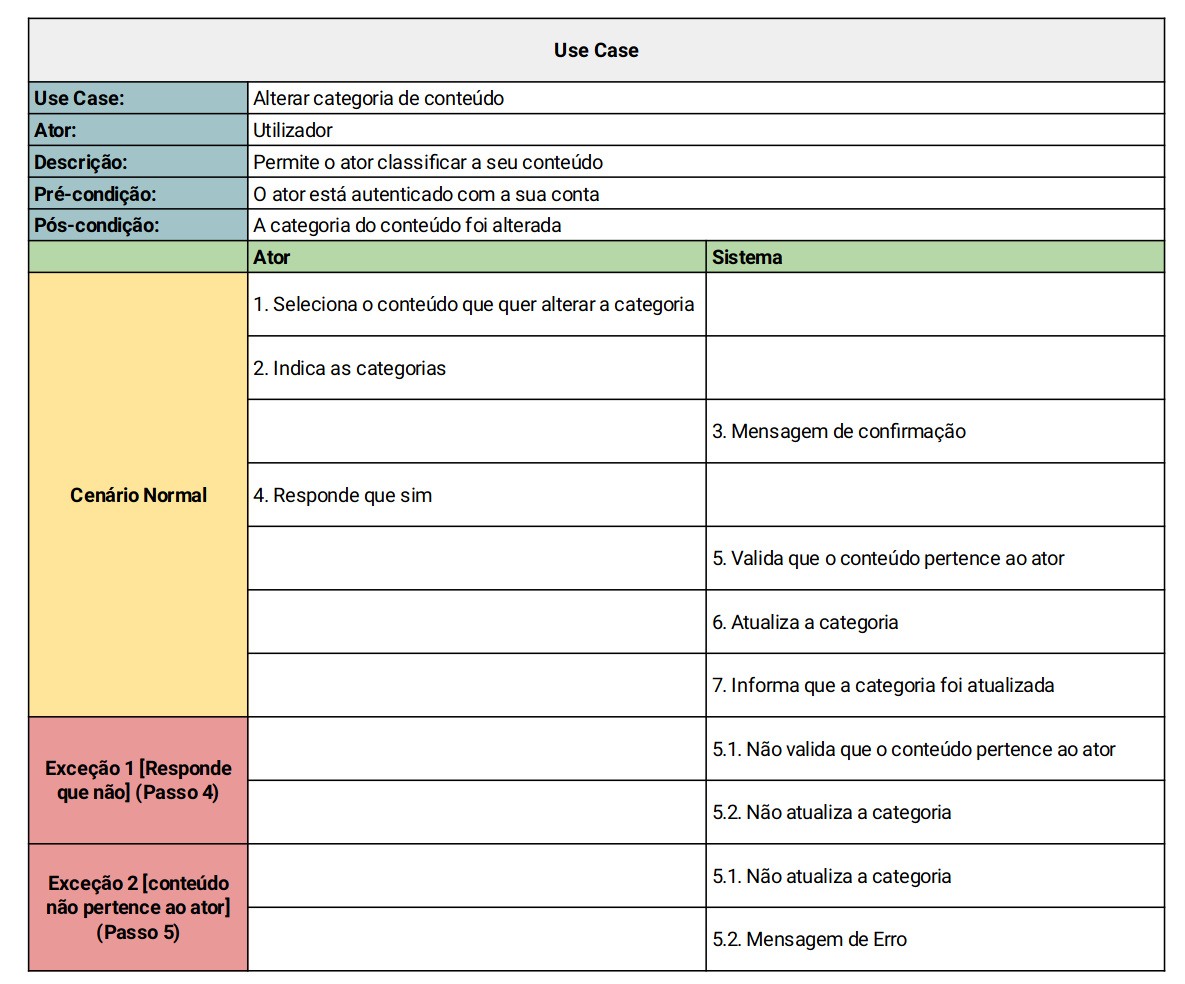
\includegraphics[width=\textwidth]{images/Classificar.png}  
    \caption{Especificação do \emph{Use Case} Alterar Categoria}
\end{figure}

\subsection{Criar Playlist}

\begin{figure}[H]
	\centering 
    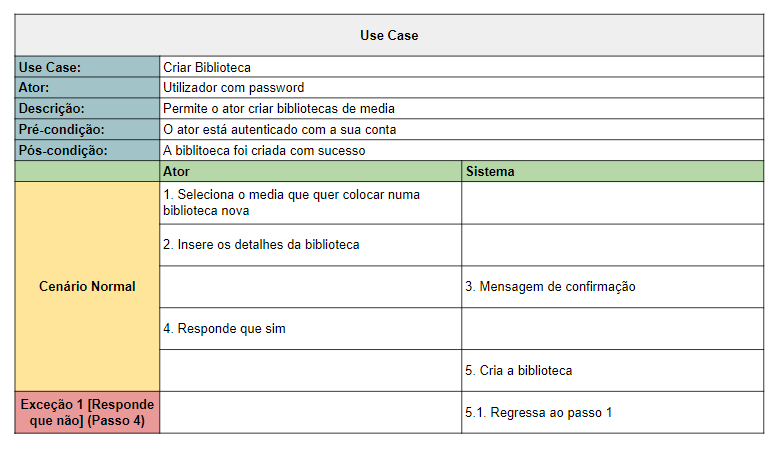
\includegraphics[width=\textwidth]{images/Criar_Biblioteca.png}  
    \caption{Especificação do \emph{Use Case} Criar Playlist}
\end{figure}

\subsection{Remover Playlist}

\begin{figure}[H]
	\centering 
    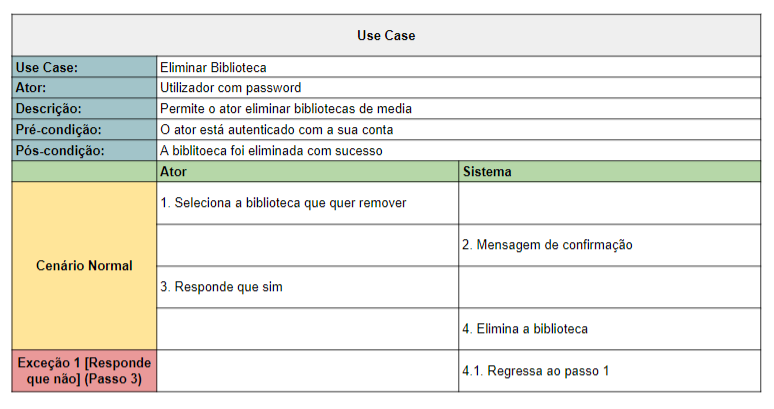
\includegraphics[width=\textwidth]{images/Eliminar_Biblioteca.png}  
    \caption{Especificação do \emph{Use Case} Remover Playlist}
\end{figure}

\subsection{Fazer convite}

\begin{figure}[H]
	\centering 
    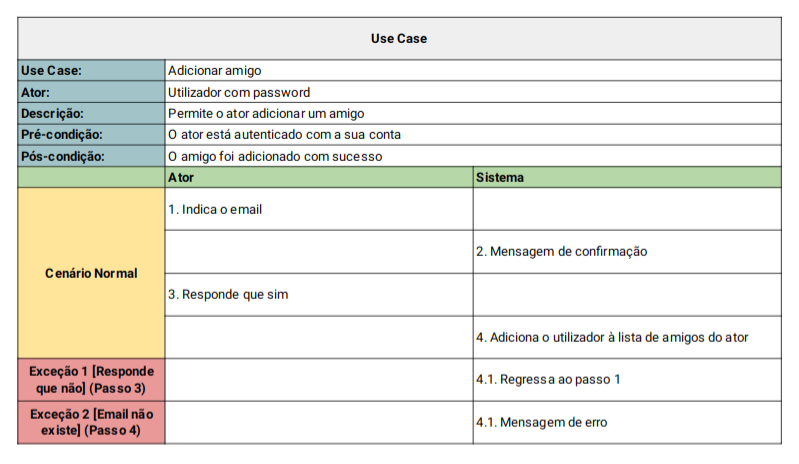
\includegraphics[width=\textwidth]{images/Adicionar_Amigo.png}  
    \caption{Especificação do \emph{Use Case} Fazer convite}
\end{figure}

\subsection{Responder convite}

\begin{figure}[H]
	\centering 
    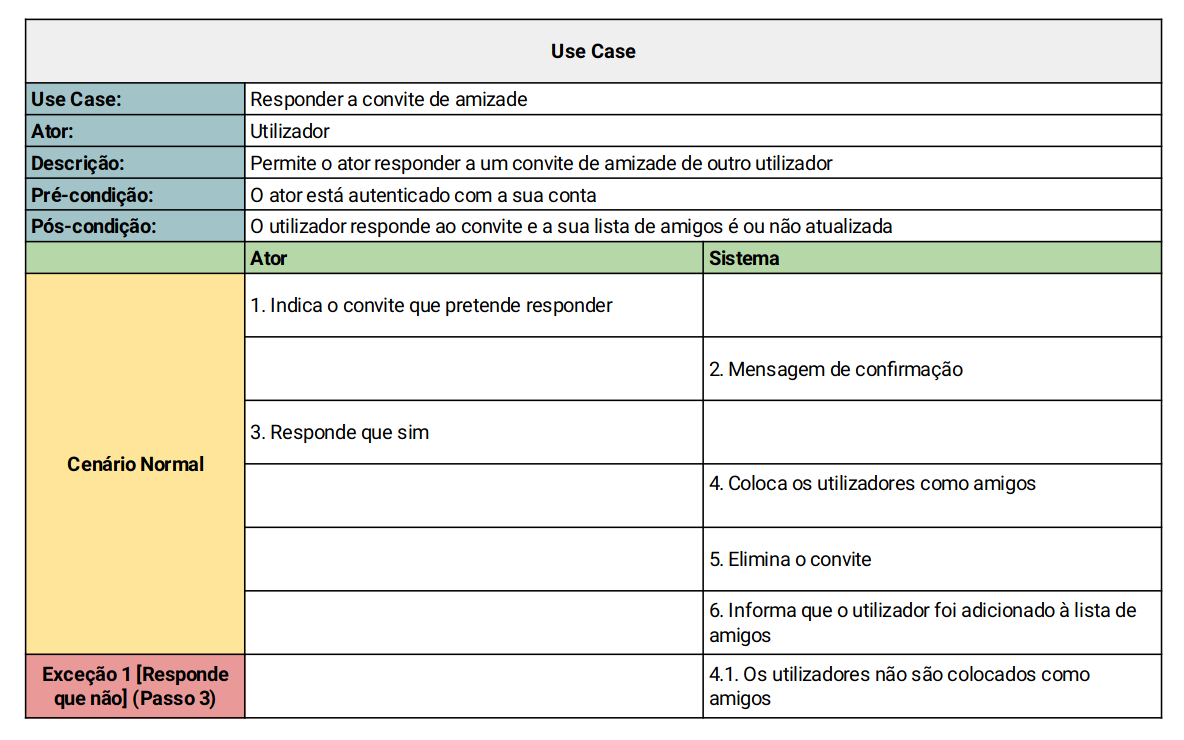
\includegraphics[width=\textwidth]{images/Responder_Convite.png}  
    \caption{Especificação do \emph{Use Case} Responder convite}
\end{figure}

\subsection{Remover amigo}

\begin{figure}[H]
	\centering 
    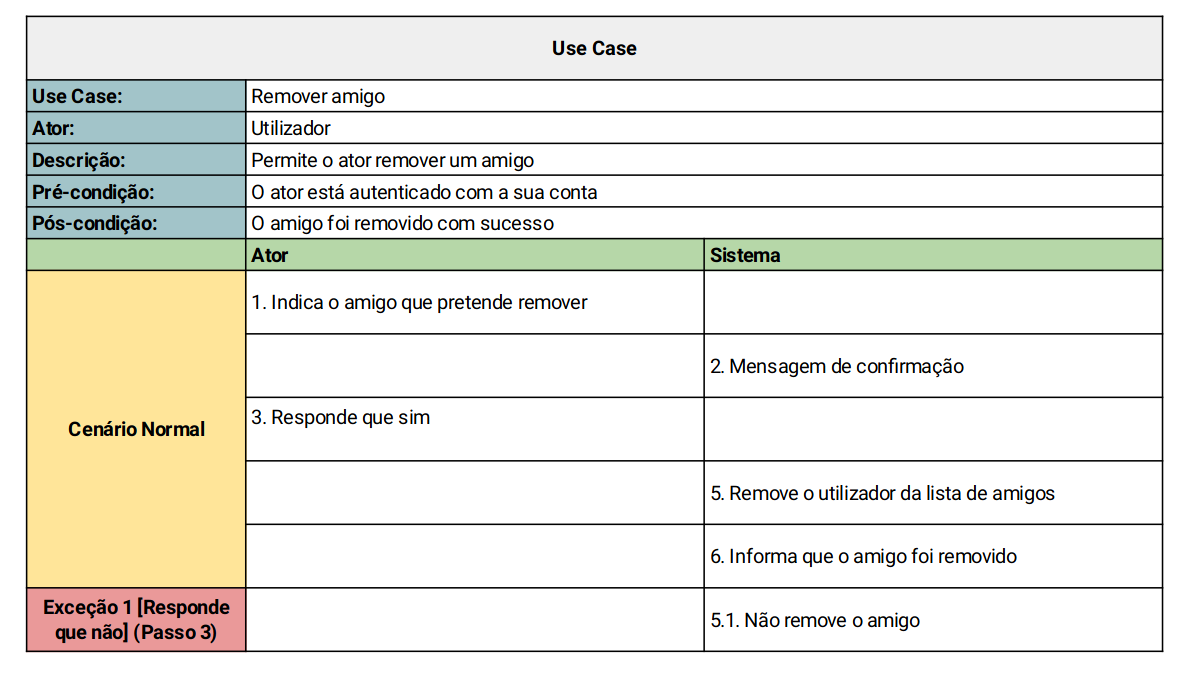
\includegraphics[width=\textwidth]{images/Remover_Amigo.png}  
    \caption{Especificação do \emph{Use Case} Remover amigo}
\end{figure}

\subsection{Registar Utilizador}

\begin{figure}[H]
	\centering 
    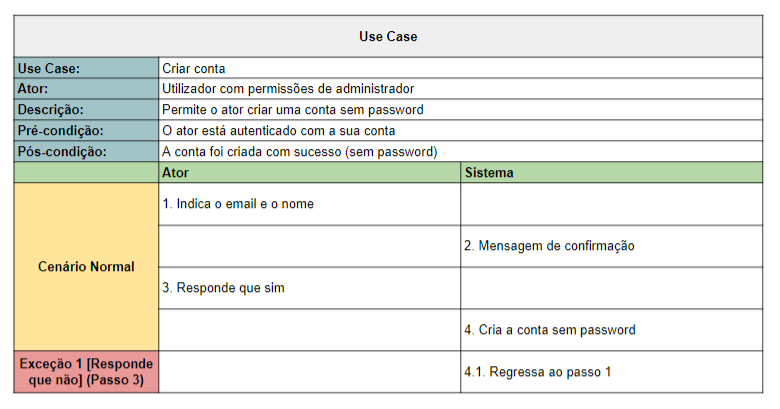
\includegraphics[width=\textwidth]{images/Criar_Conta.png}  
    \caption{Especificação do \emph{Use Case} Registar Utilizador}
\end{figure}

\subsection{Eliminar utilizador}

\begin{figure}[H]
	\centering 
    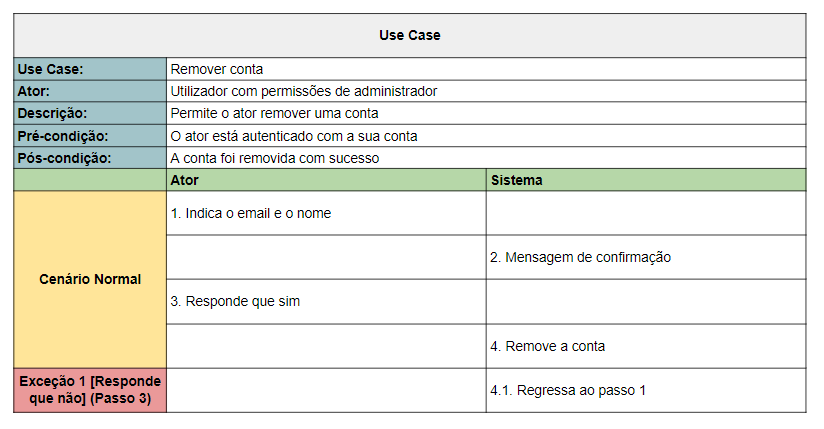
\includegraphics[width=\textwidth]{images/Remover_Conta.png}  
    \caption{Especificação do \emph{Use Case} Eliminar Utilizador}
\end{figure}

\chapter{Mockups}

\textit{Mockups} é o nome dado aos protótipos de interface.\\
Como o próprio nome indica é uma demonstração de como a aplicação final vai
ser.\\
O principal foco da equipa foi desenvolver um \textit{design} moderno e
intuitivo mantendo uma aparência simples e visualmente apelativa.\\
A fim de explorar as linhas de design modernas, decidimos criar um
\textit{design} mais escuro, normalmente denominado de \textit{darkmode}. Para
além de ter um aspeto mais moderno e futurista, o \textit{darkmode} permite uma
menor fadiga ocular, e caso o ecrã onde o conteúdo esteja a ser visualizado seja
OLED ou AMOLED, um menor consumo de energia.

\section{Sem sessão iniciada}

\begin{figure}[H]
	\centering 
    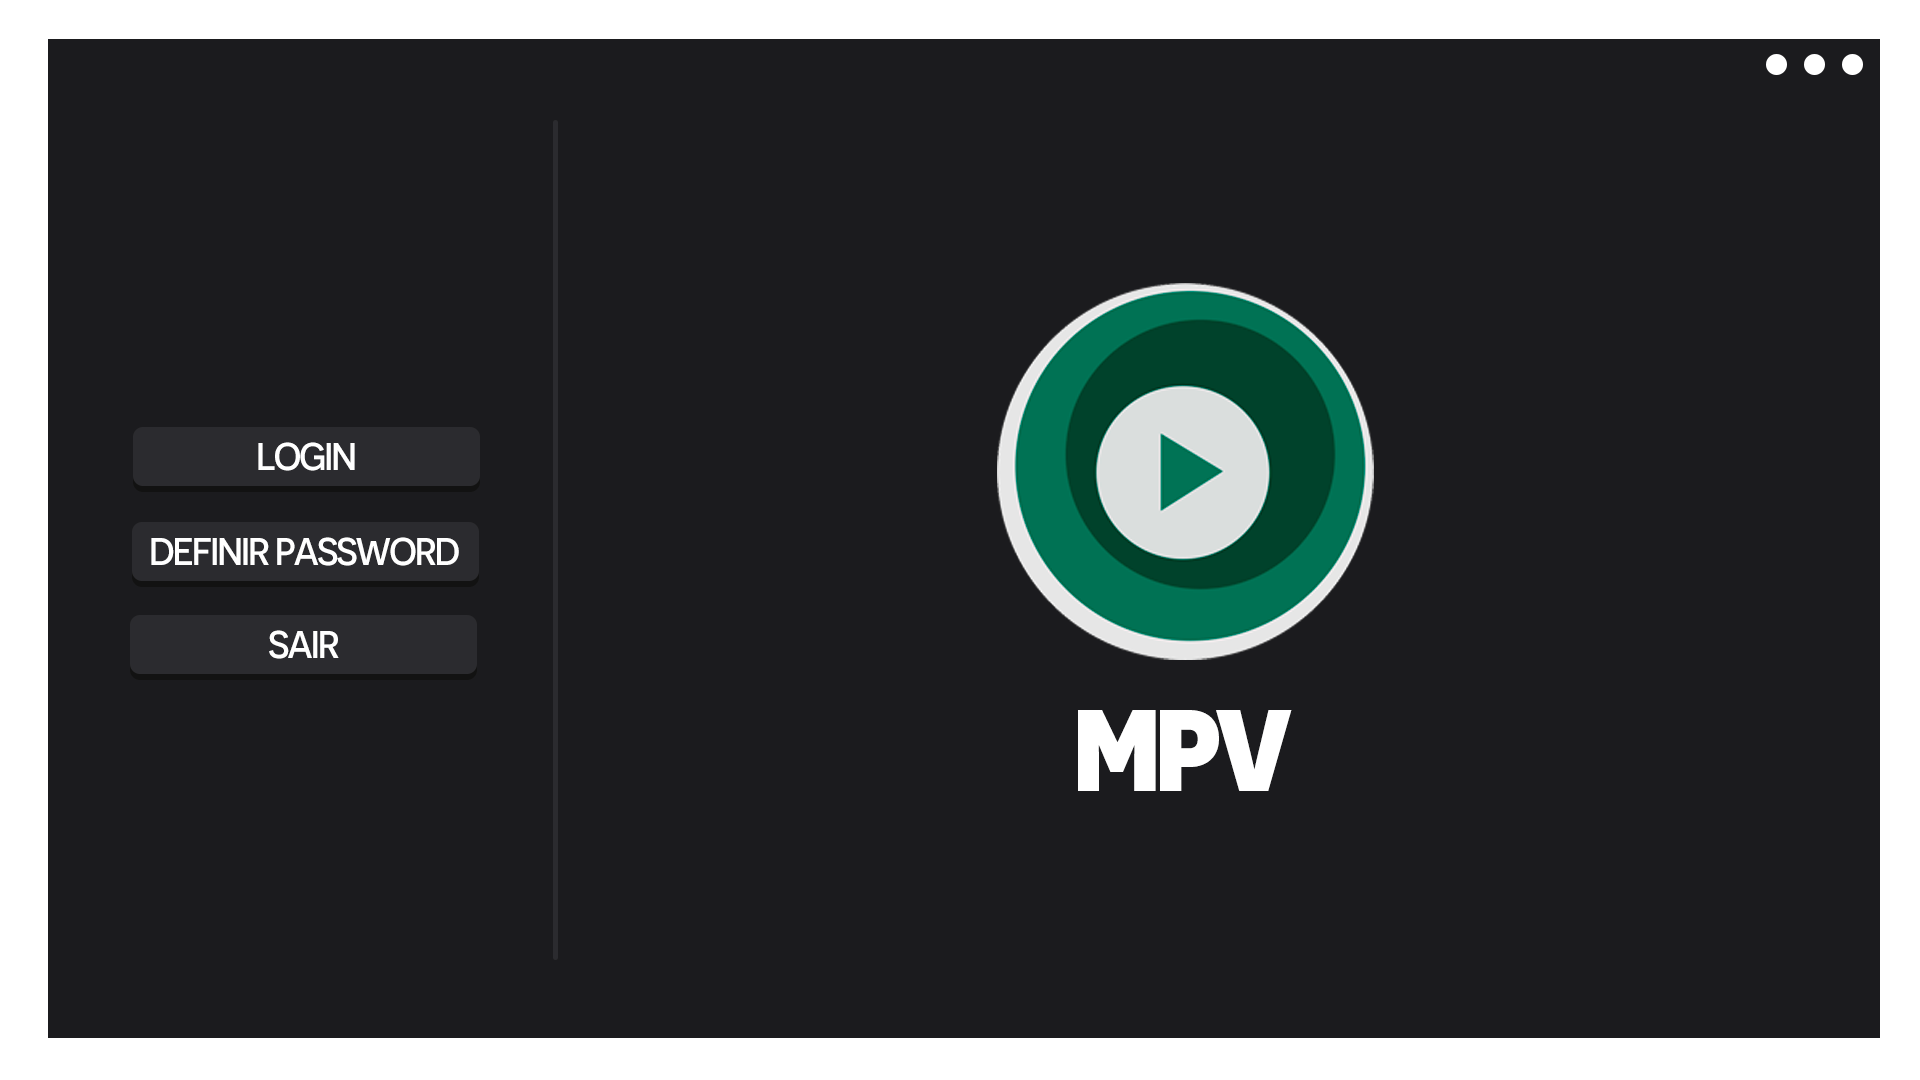
\includegraphics[width=\textwidth]{images/Inicio_Menu.png}  
    \caption{Menu inicial}
\end{figure}

\begin{figure}[H]
	\centering 
    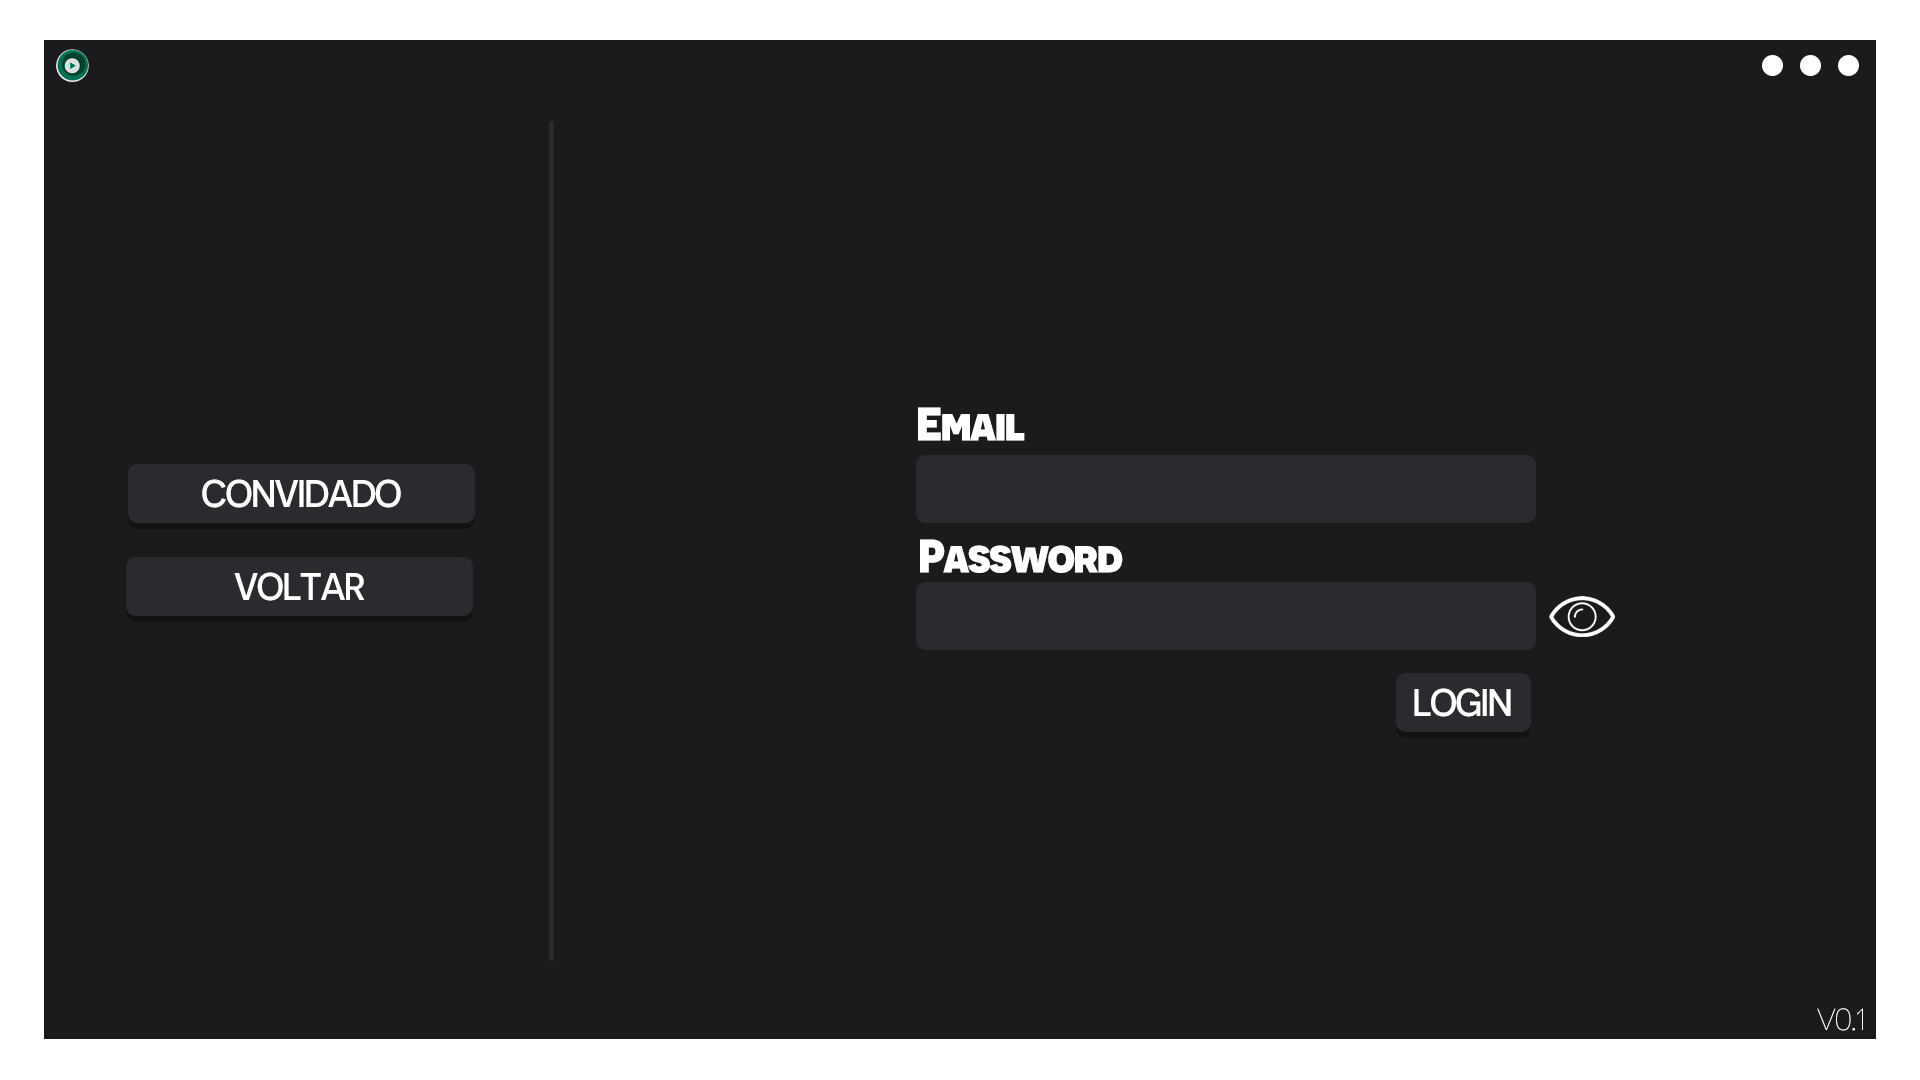
\includegraphics[width=\textwidth]{images/Login_Menu.png}  
    \caption{Login}
\end{figure}

\begin{figure}[H]
	\centering 
    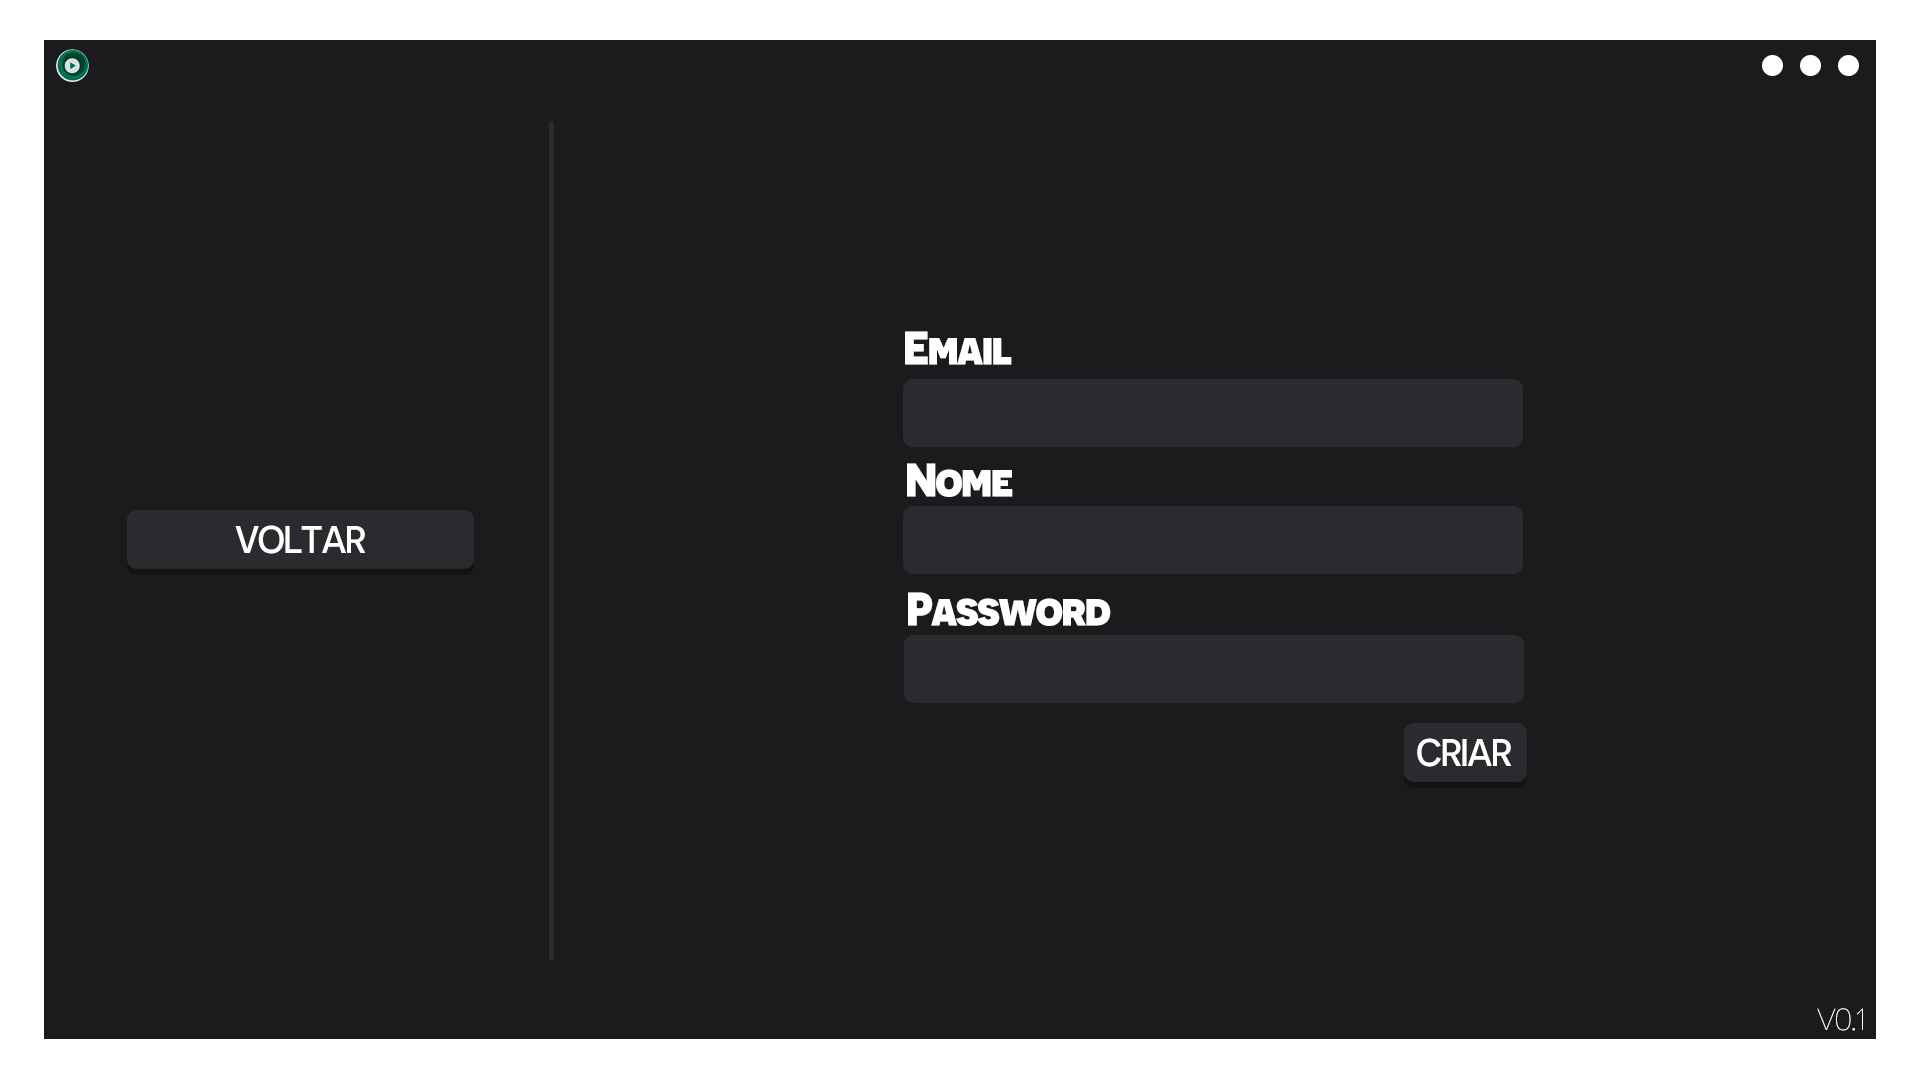
\includegraphics[width=\textwidth]{images/DefinirPassword_Menu.png}  
    \caption{Definir password para os utilizadores sem password a definirem}
\end{figure}

\begin{figure}[H]
	\centering 
    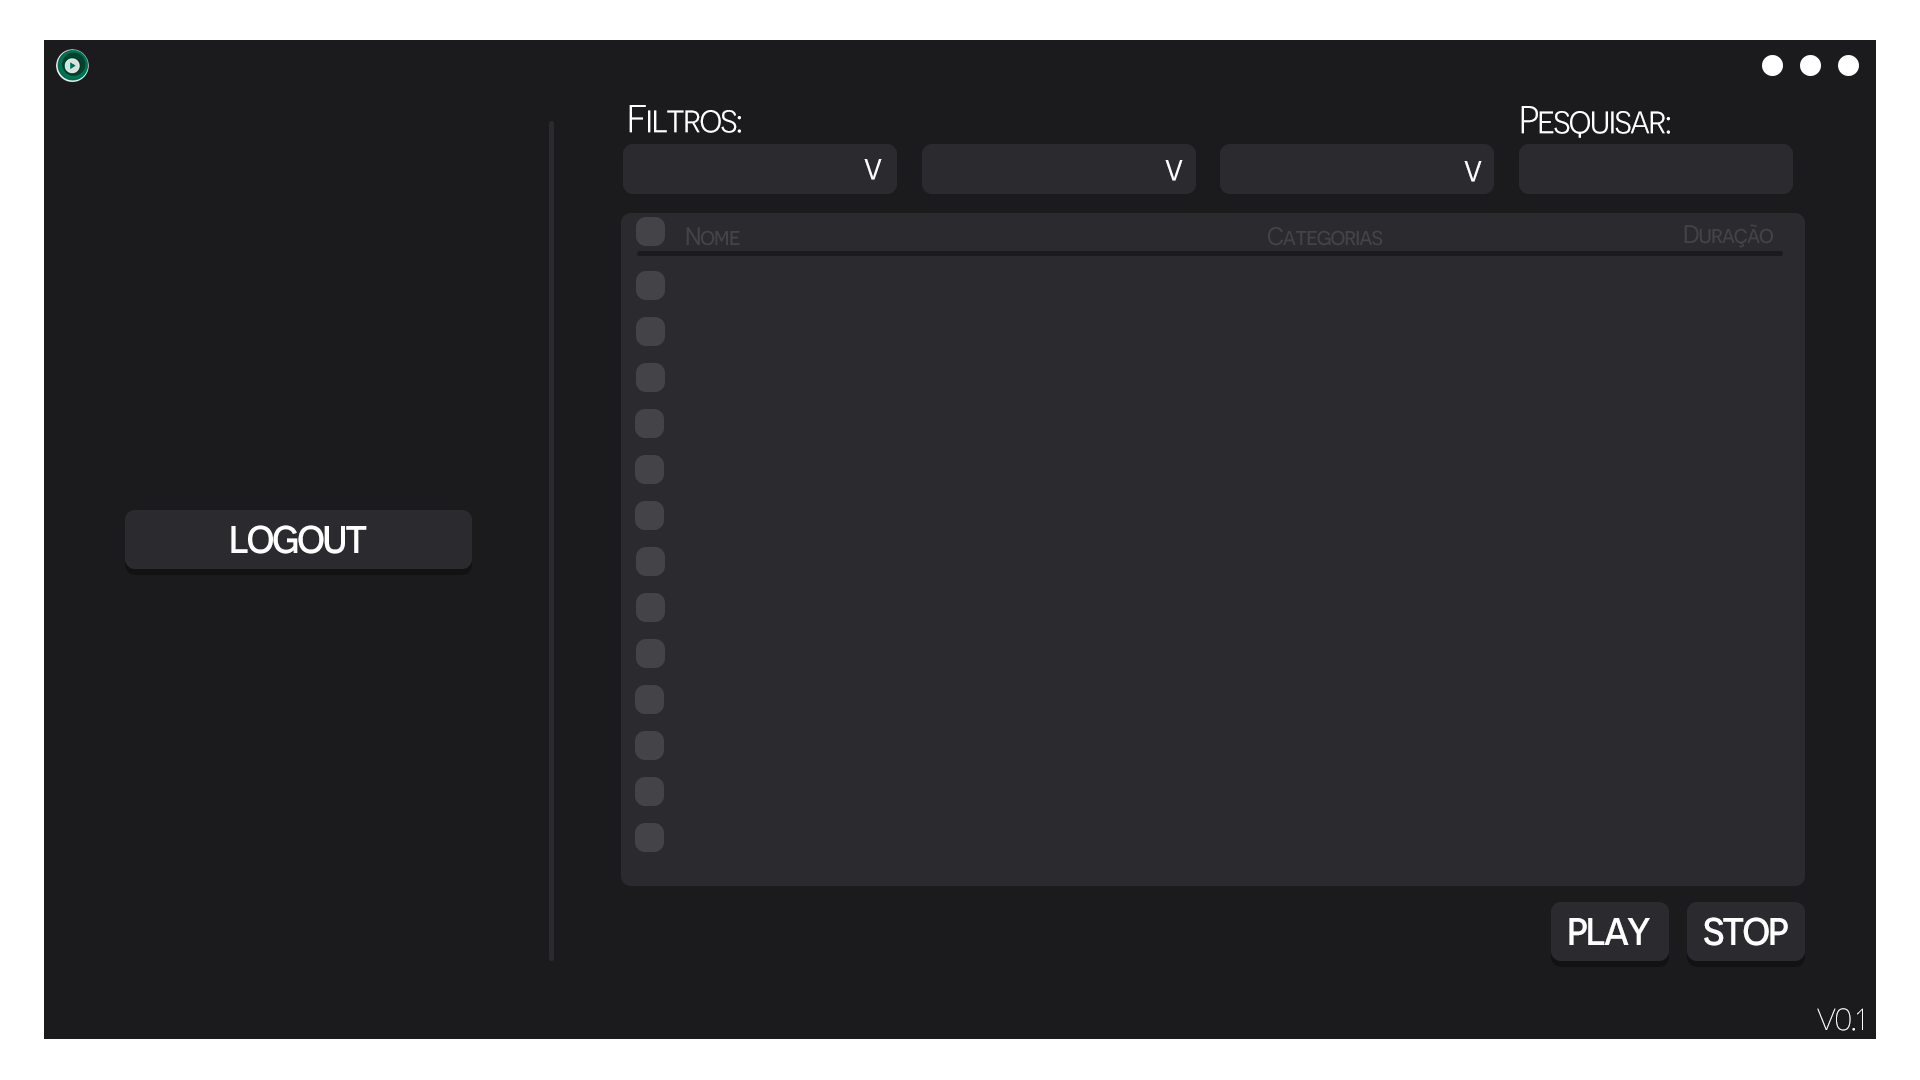
\includegraphics[width=\textwidth]{images/Principal_convidado_Menu.png}  
    \caption{Menu para um utilizador que entrou como convidado}
\end{figure}

\section{Com sessão iniciada}

\begin{figure}[H]
	\centering 
    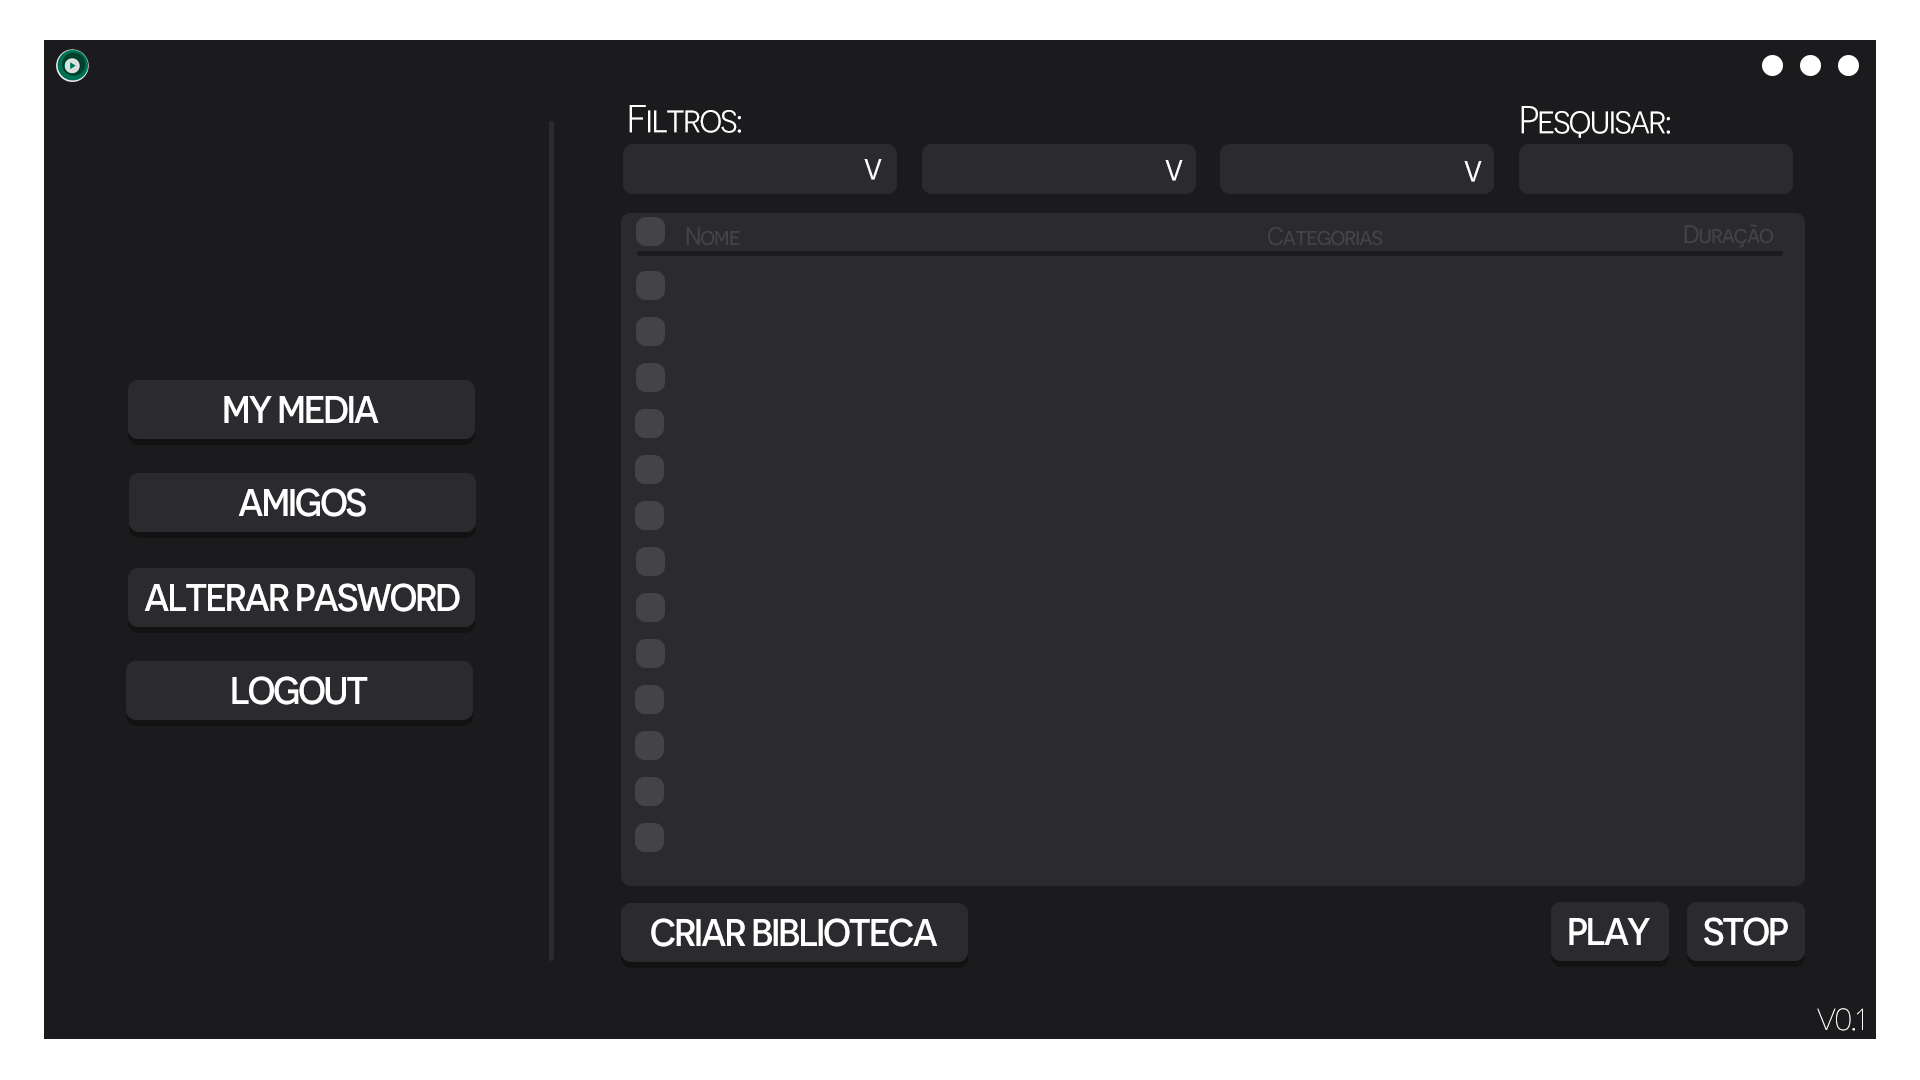
\includegraphics[width=\textwidth]{images/Principal_Menu.png}  
    \caption{Menu para um utilizador autenticado com password}
\end{figure}

\begin{figure}[H]
	\centering 
    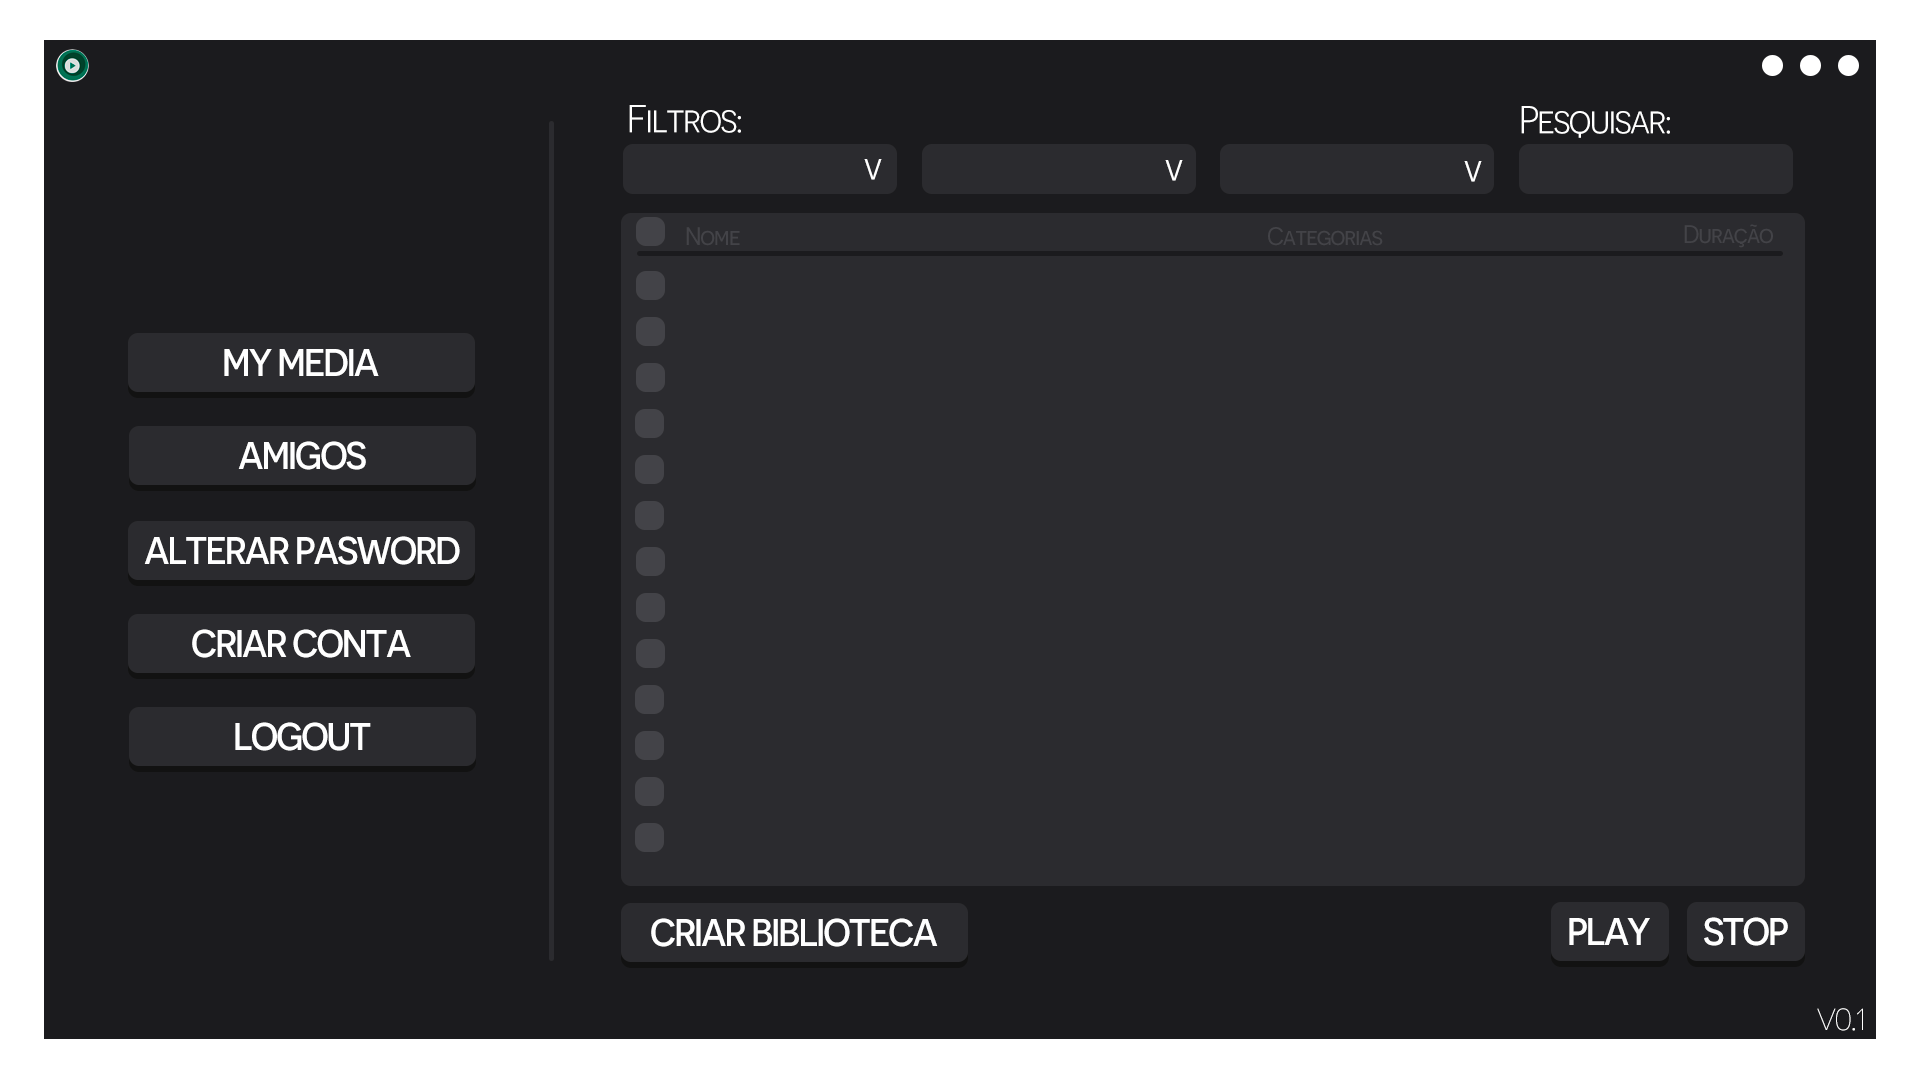
\includegraphics[width=\textwidth]{images/Principal_Admin_Menu.png}  
    \caption{Menu para um utilizador com permissões de administrador autenticado}
\end{figure}

\begin{figure}[H]
	\centering 
    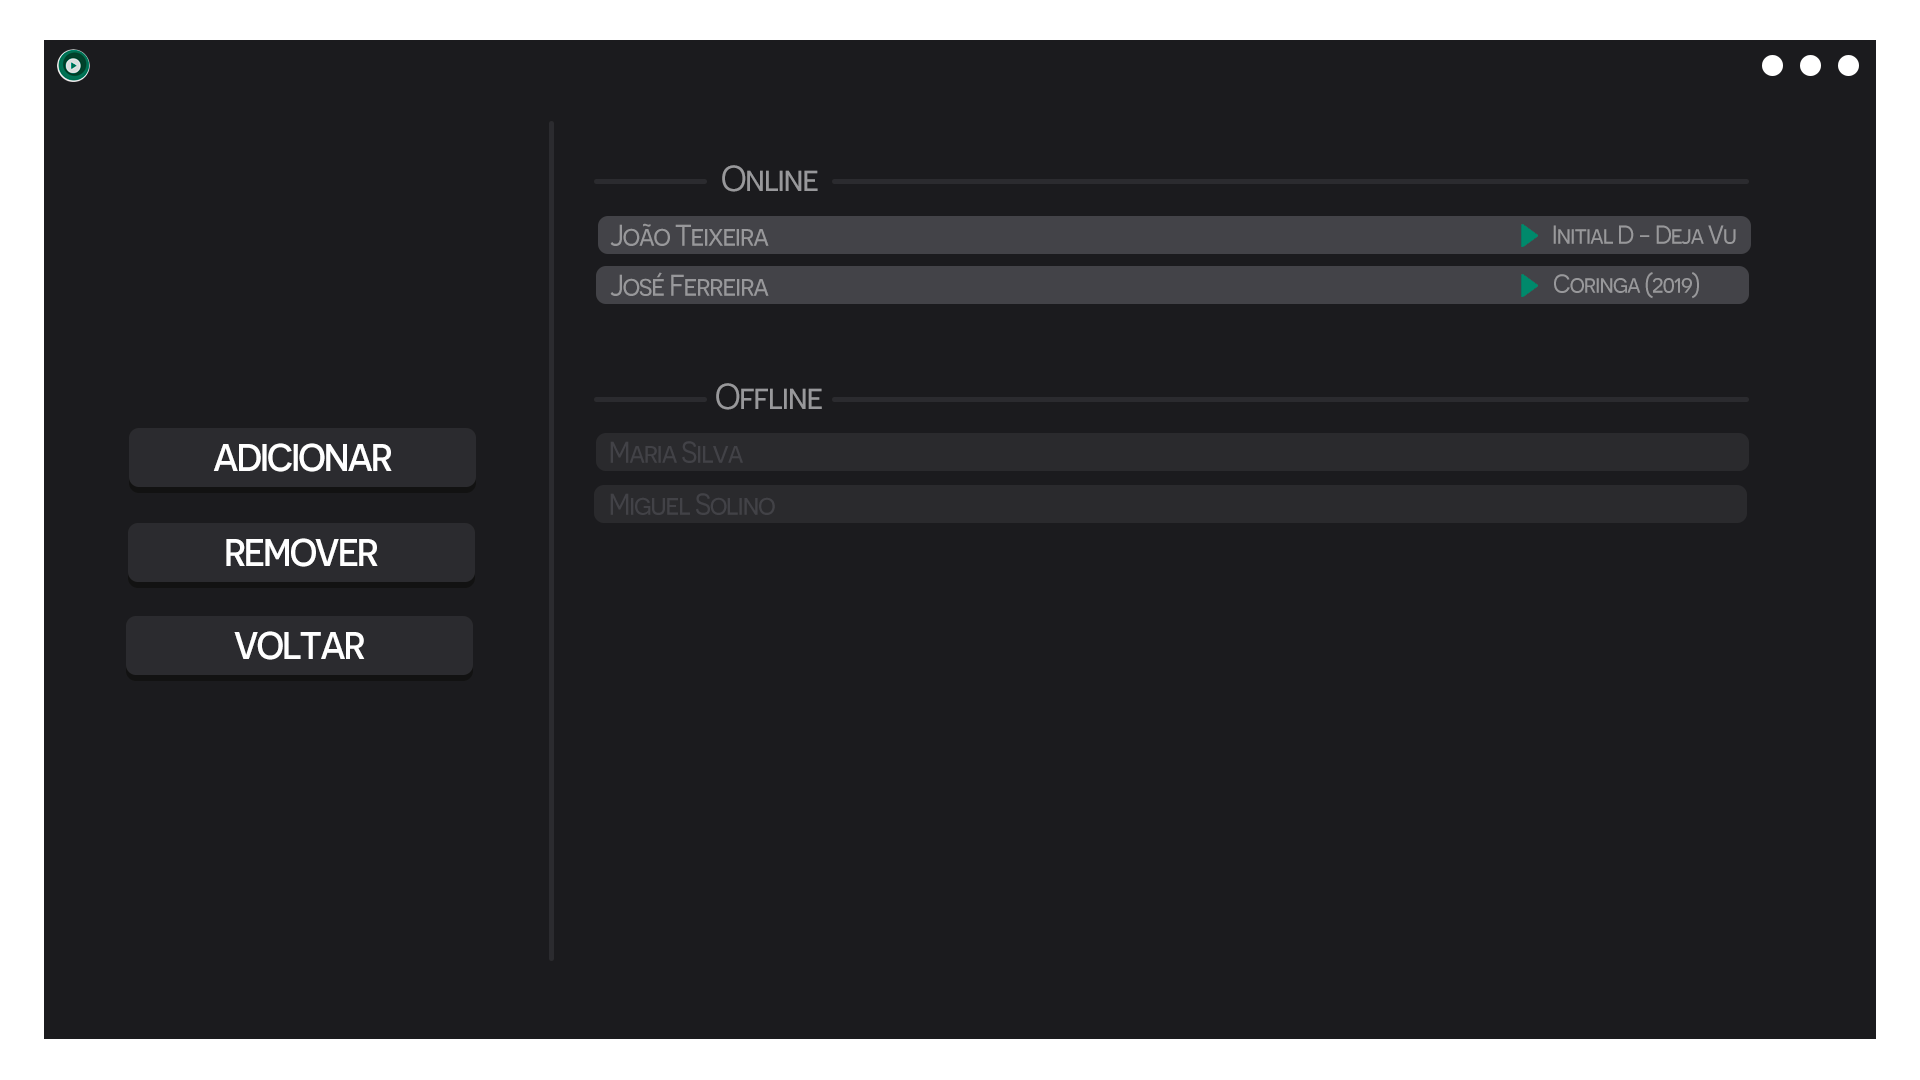
\includegraphics[width=\textwidth]{images/Amigos_Menu.png}  
    \caption{Menu com as amizades}
\end{figure}

\begin{figure}[H]
	\centering 
    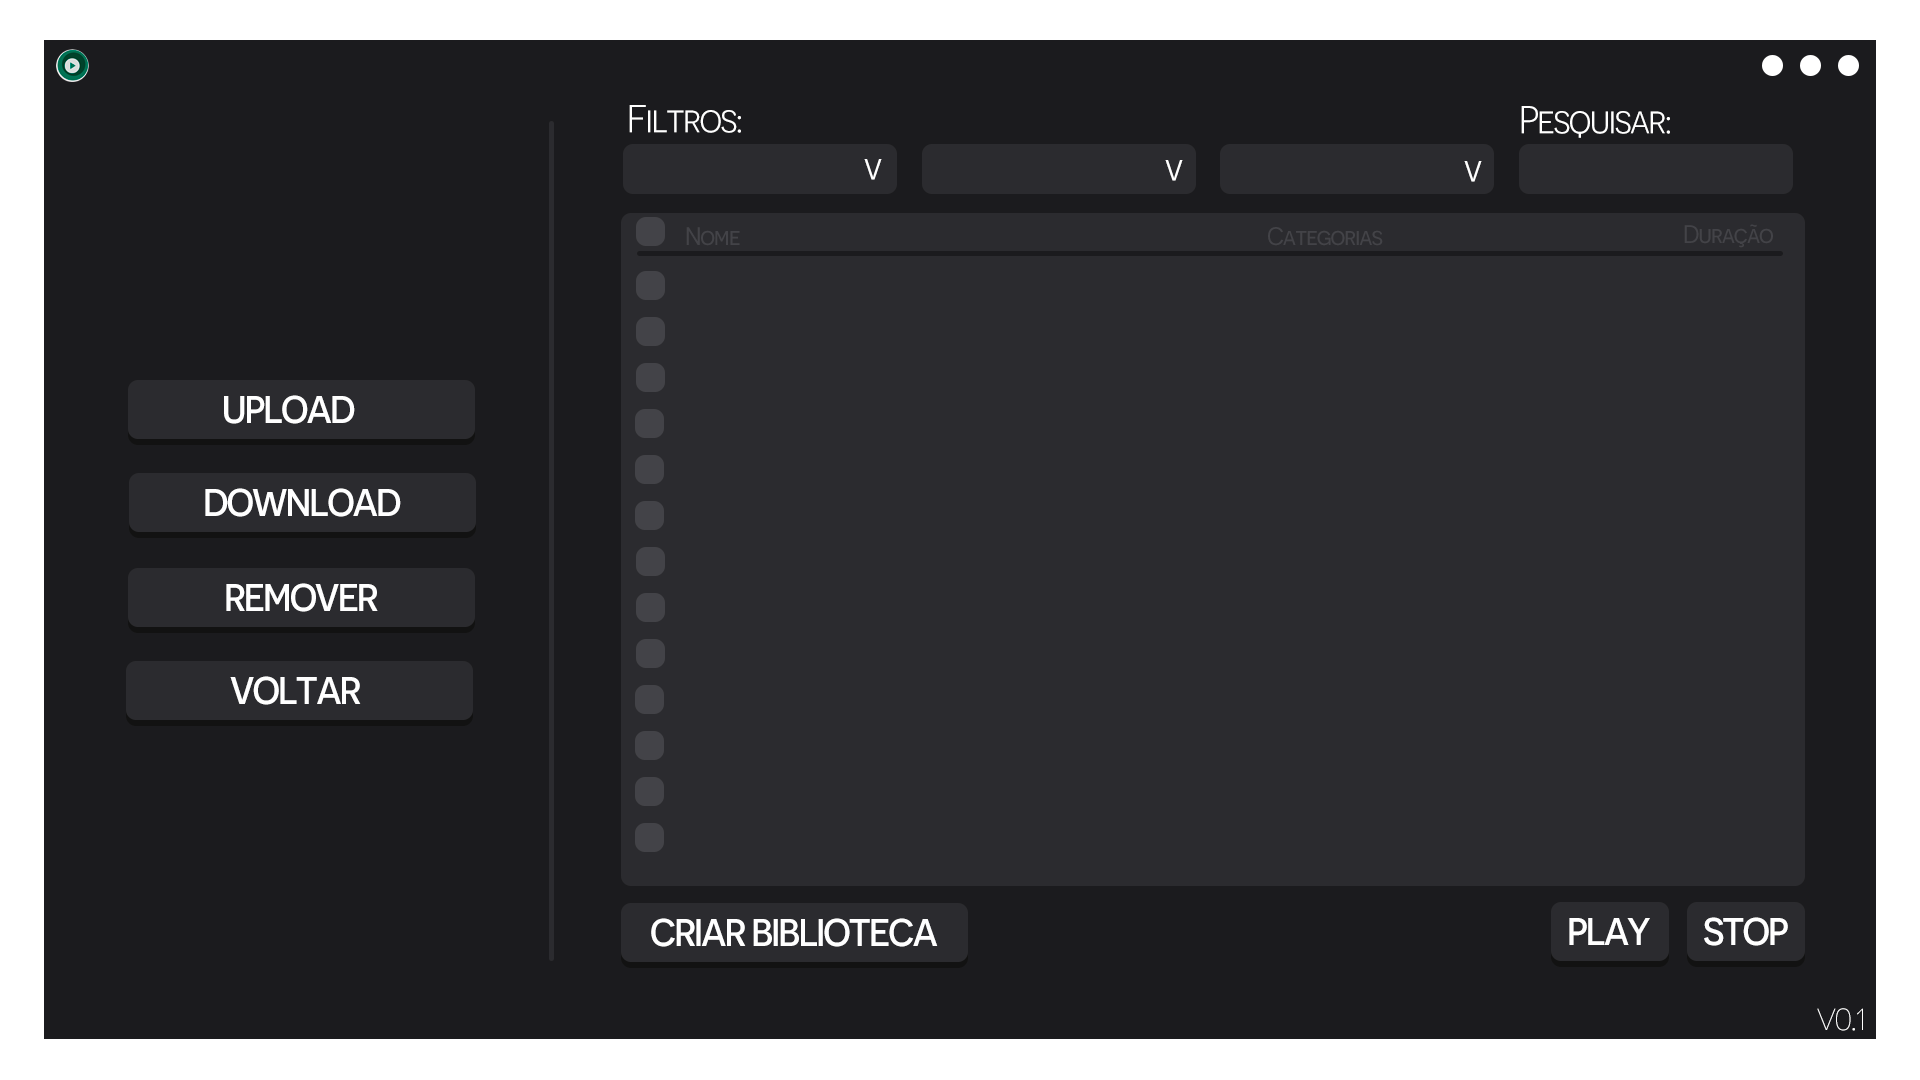
\includegraphics[width=\textwidth]{images/MyMedia_Menu.png}  
    \caption{Menu com a media do utilizador autenticado}
\end{figure}

\begin{figure}[H]
	\centering 
    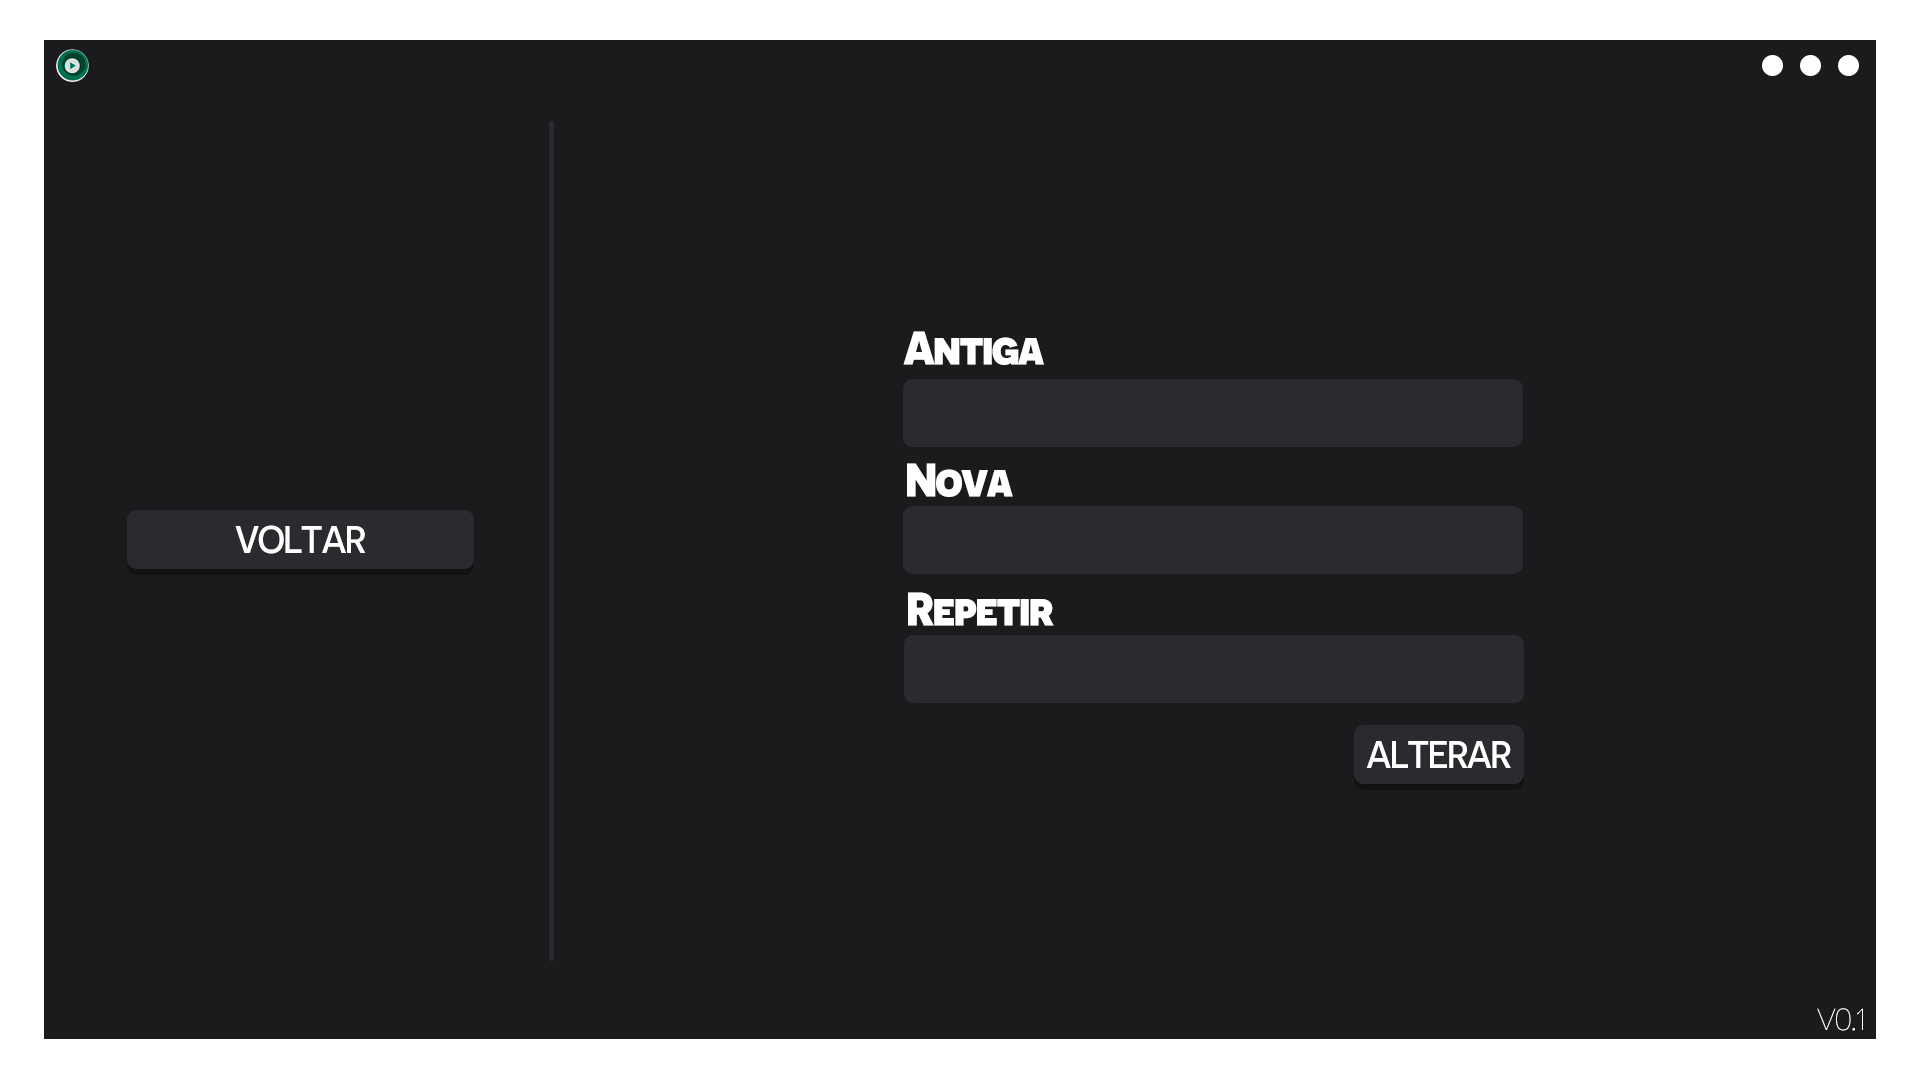
\includegraphics[width=\textwidth]{images/AlterarPassword_Menu.png}  
    \caption{Menu para alterar a password}
\end{figure}

\begin{figure}[H]
	\centering 
    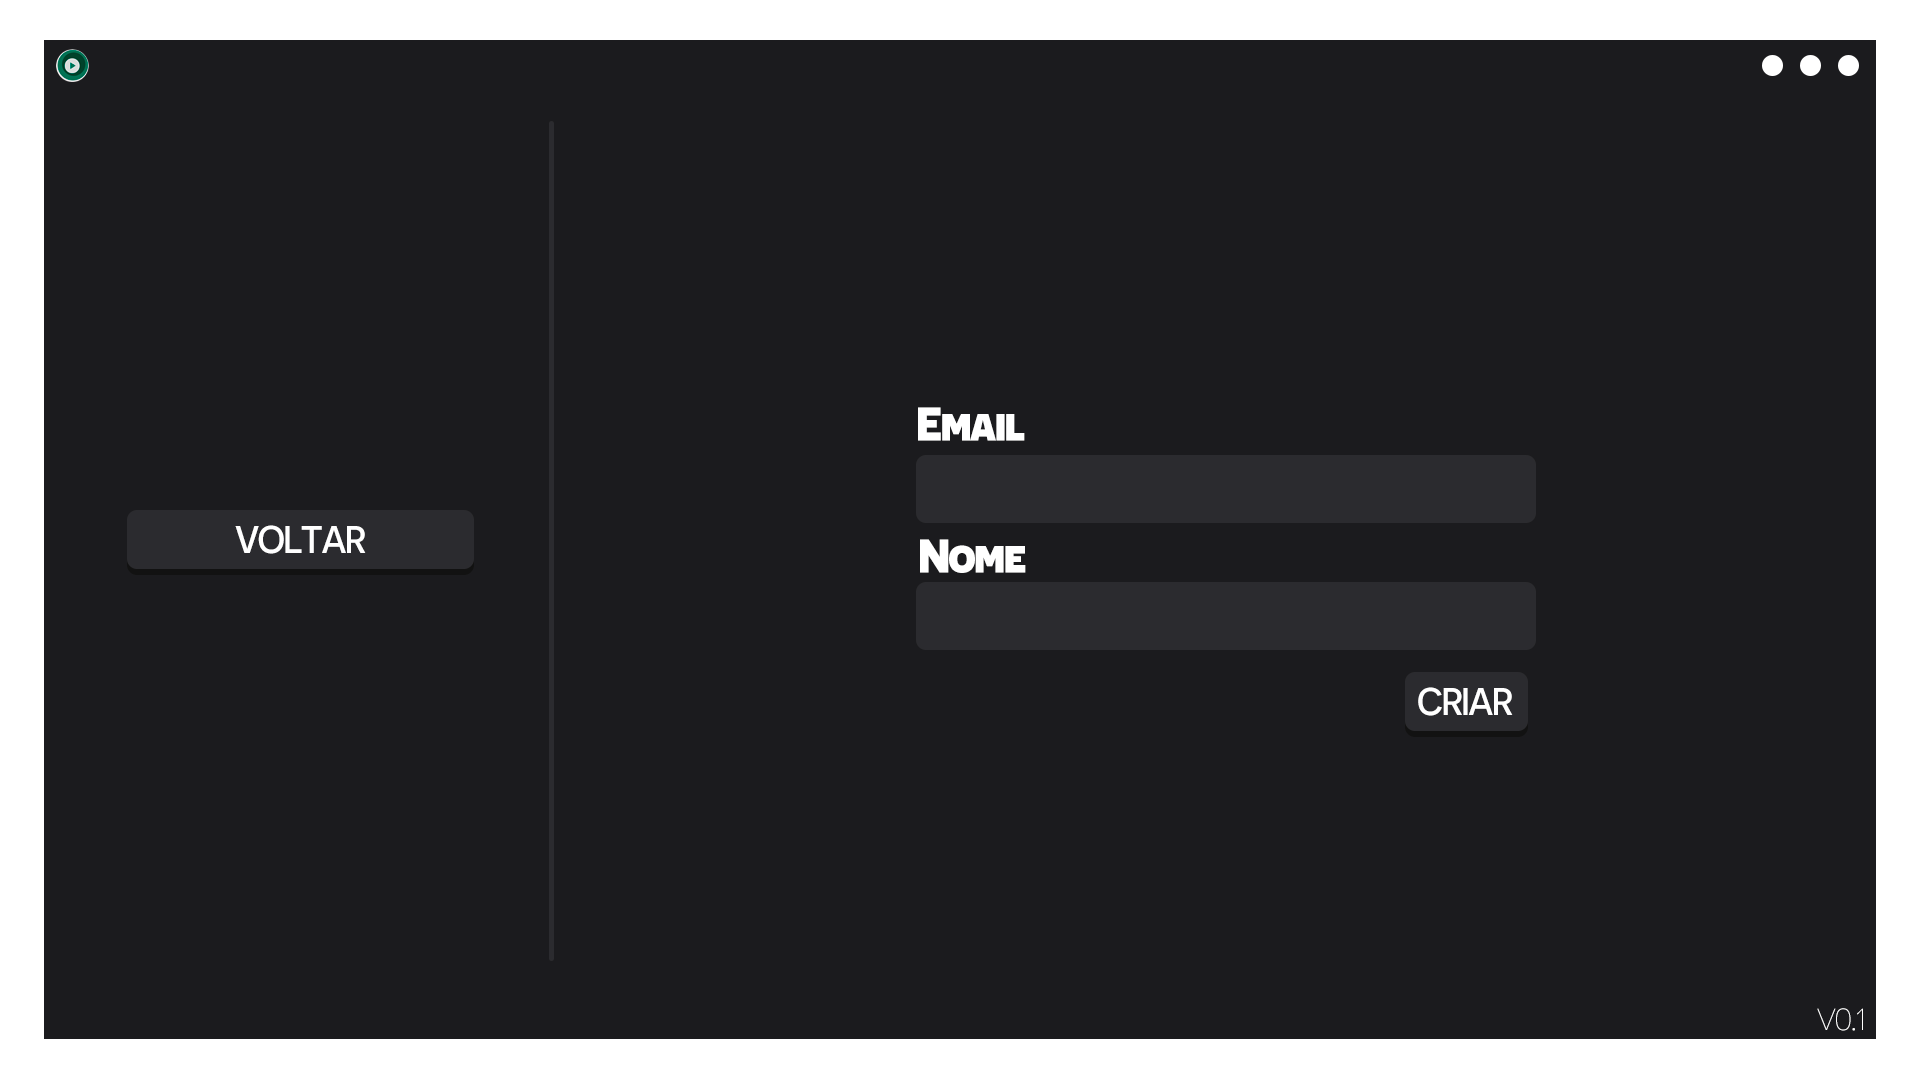
\includegraphics[width=\textwidth]{images/CriarConta_Menu.png}  
    \caption{Menu para utilizadores com permissões de administrador criarem contas sem password}
\end{figure}

\begin{figure}[H]
	\centering 
    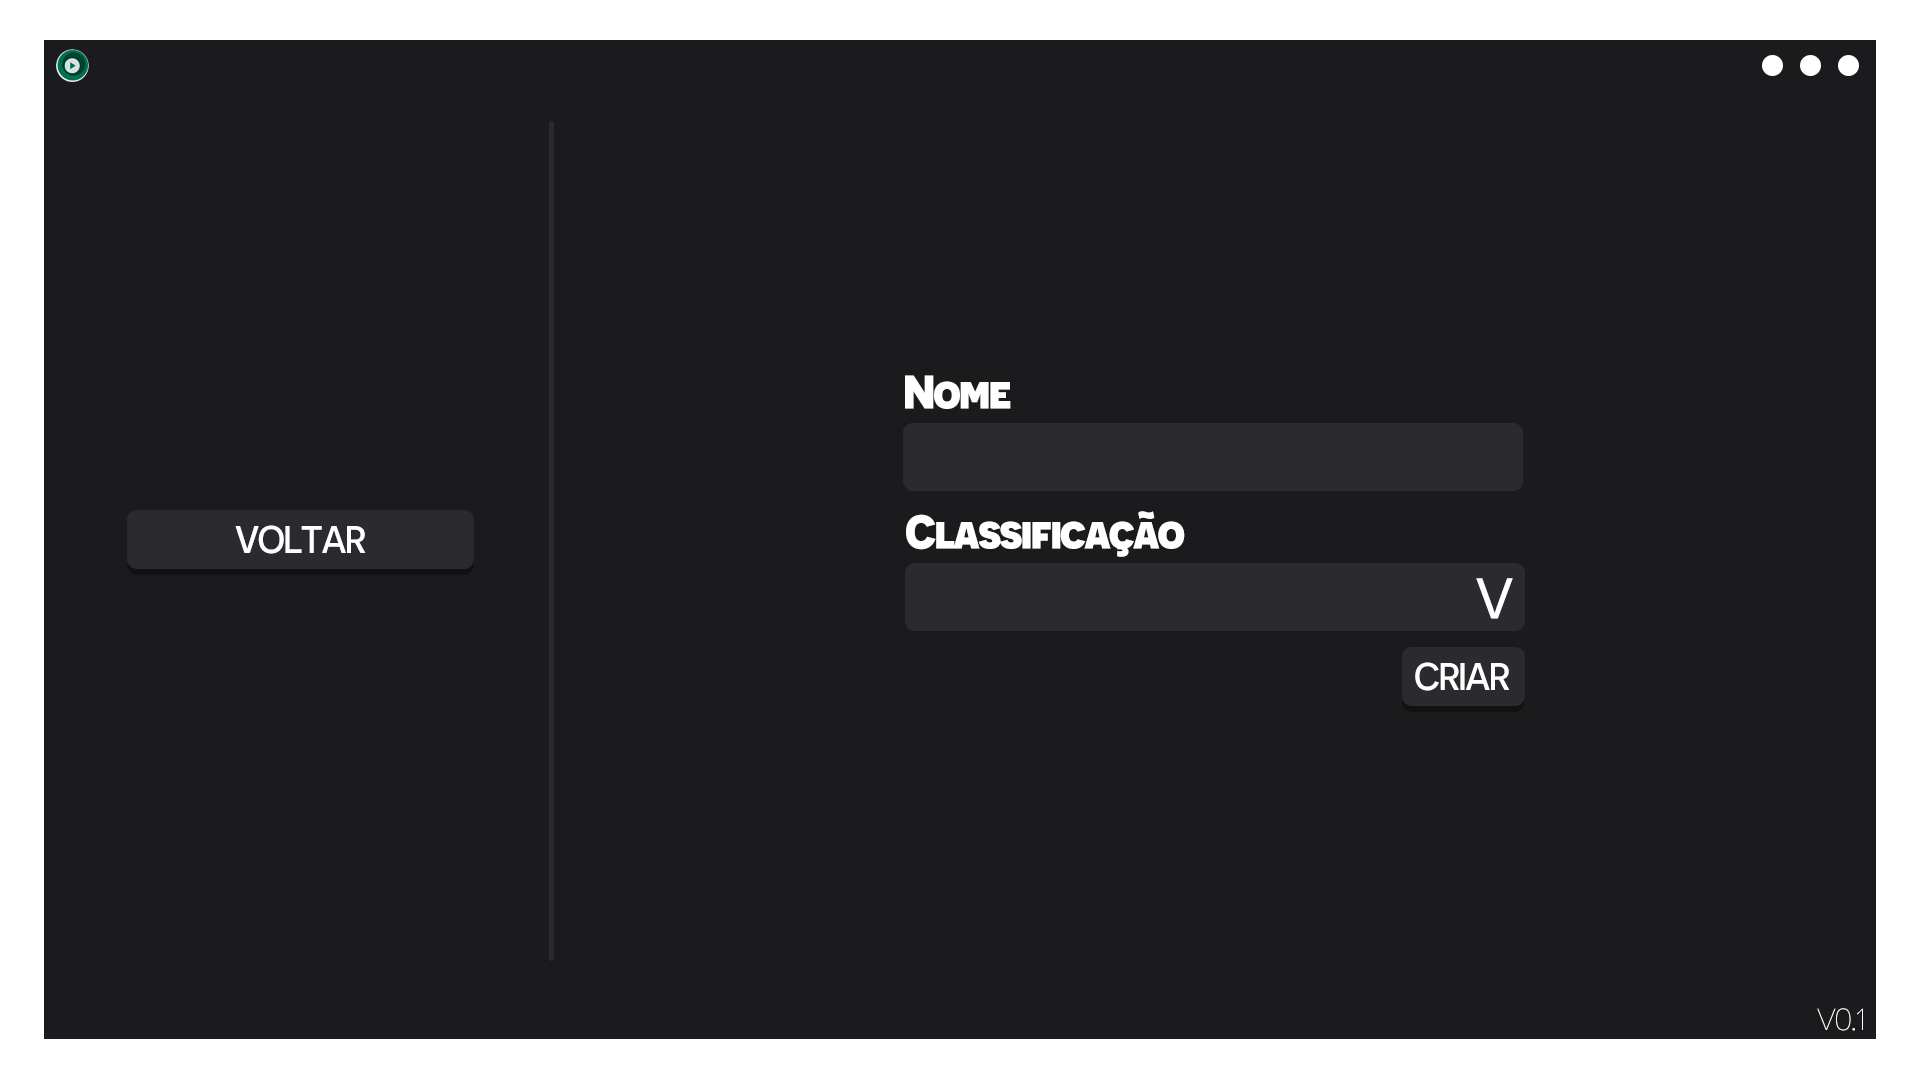
\includegraphics[width=\textwidth]{images/Criar_Biblioteca_Menu.png}  
    \caption{Menu para criar uma biblioteca}
\end{figure}

\begin{figure}[H]
	\centering 
    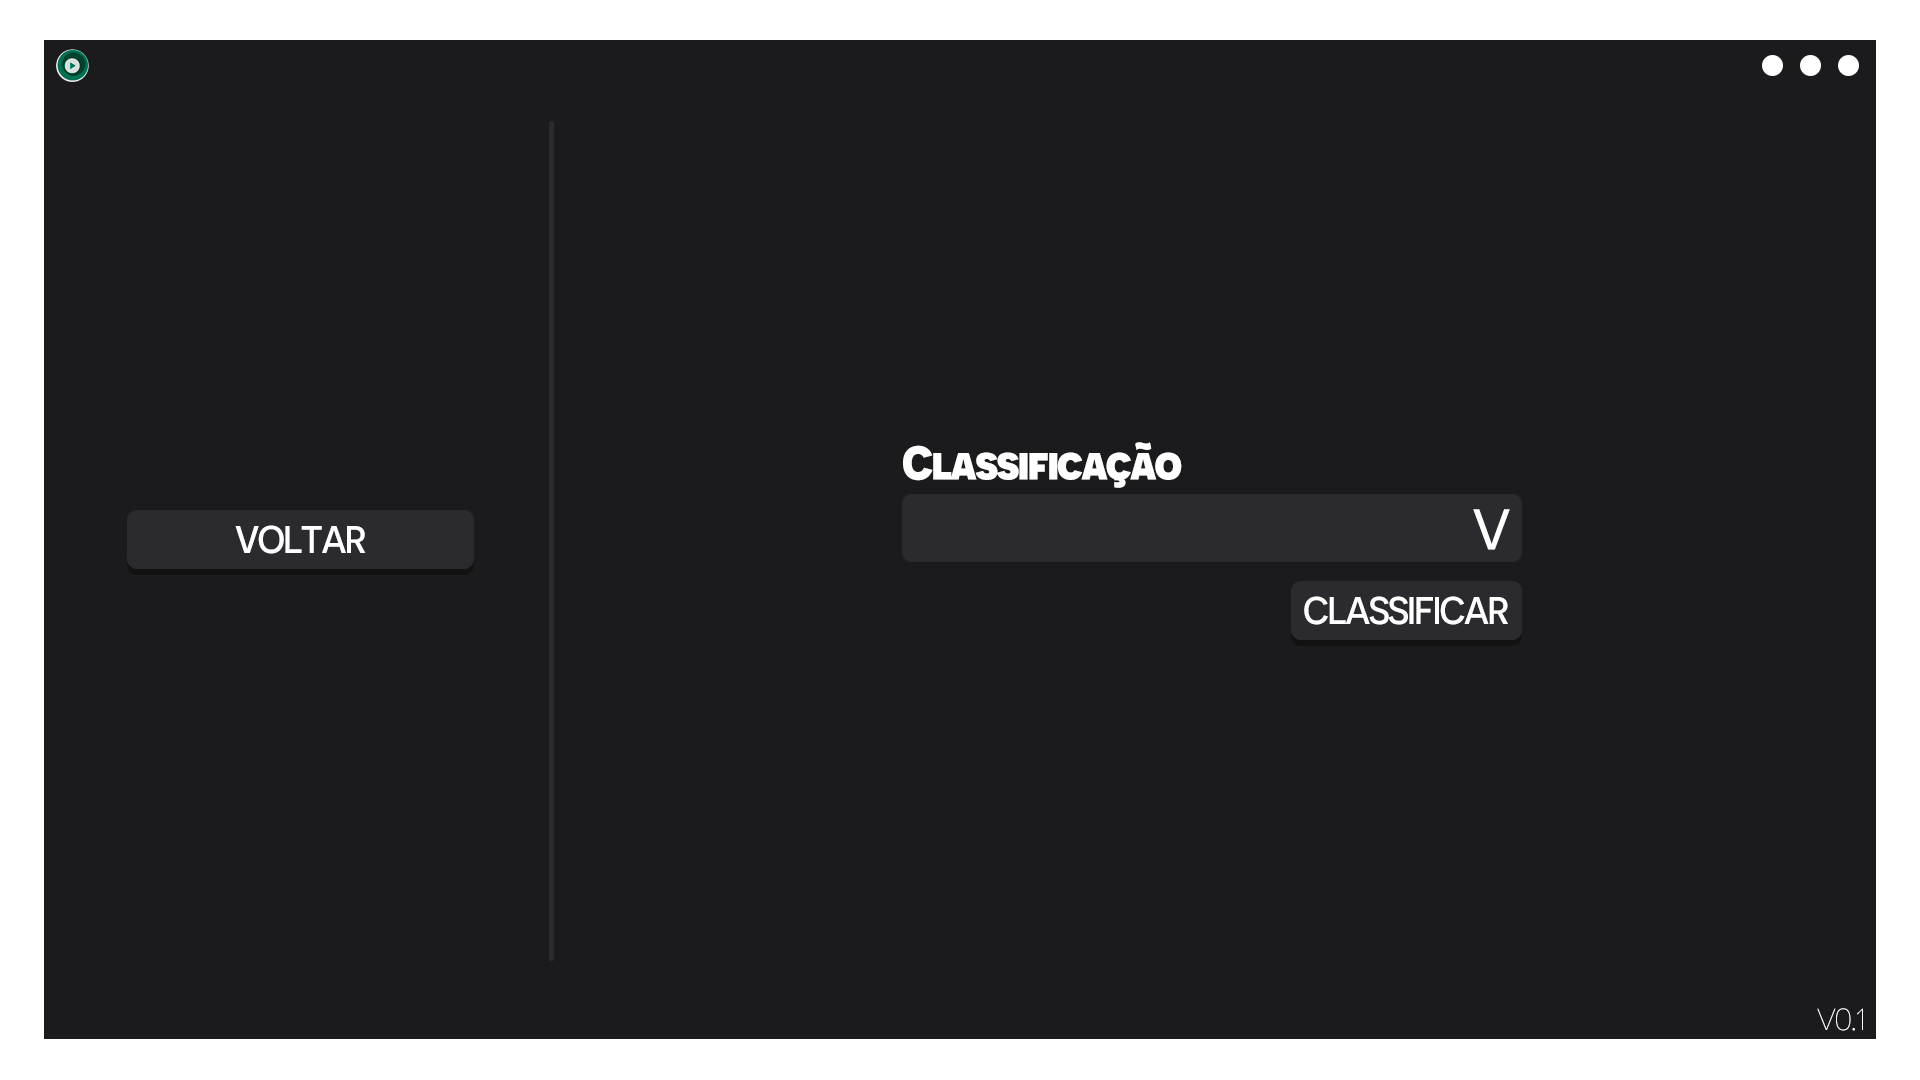
\includegraphics[width=\textwidth]{images/Classificar_Menu.png}  
    \caption{Menu para classificar um ou mais media}
\end{figure}

\chapter{Diagrama de Sequência de Sistemas}

Com base nos use cases e nas suas especificações foram construidos diagramas de sequência
para cada use case que nos ajudam a interpretar como o sistema e o ator interajem entre
si.

\section{Login}

\begin{figure}[H]
	\centering 
    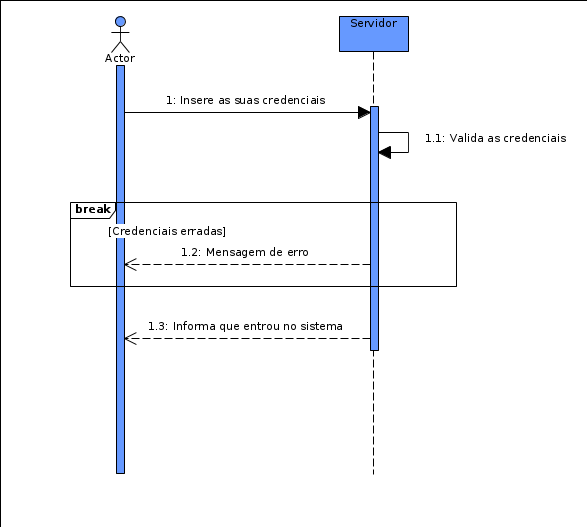
\includegraphics[width=\textwidth]{images/loginSeq.png}  
    \caption{Diagrama de sequência do Login}
\end{figure}

\section{Logout}

\begin{figure}[H]
	\centering 
    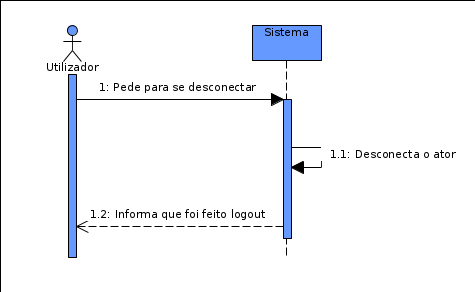
\includegraphics[width=\textwidth]{images/logoutSeq.png}  
    \caption{Diagrama de sequência do Logout}
\end{figure}

\section{Entrar como convidado}

\begin{figure}[H]
	\centering 
    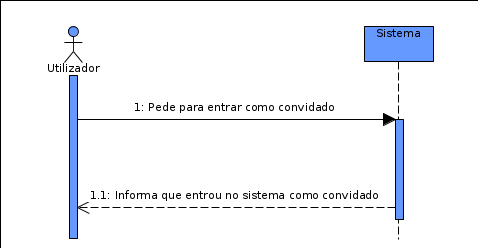
\includegraphics[width=\textwidth]{images/convidadoSeq.png}  
    \caption{Diagrama de sequência do Entrar como Convidado}
\end{figure}

\section{Upload}

\begin{figure}[H]
	\centering 
    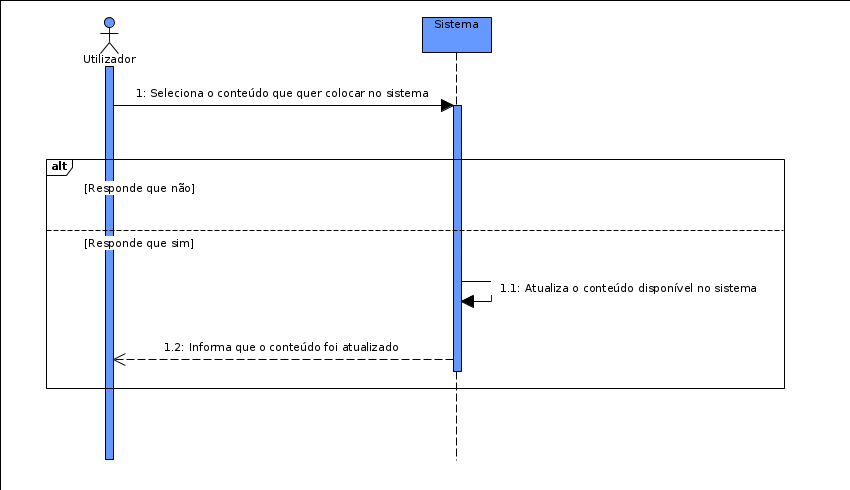
\includegraphics[width=\textwidth]{images/uploadSeq.png}  
    \caption{Diagrama de sequência do Upload}
\end{figure}

\section{Download}

\begin{figure}[H]
	\centering 
    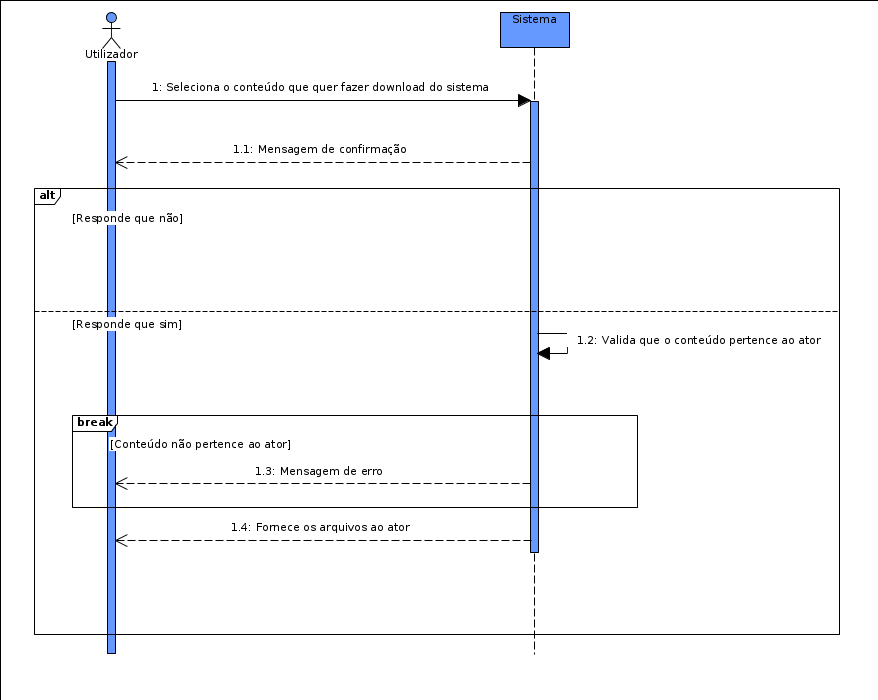
\includegraphics[width=\textwidth]{images/downloadSeq.png}  
    \caption{Diagrama de sequência do Download}
\end{figure}

\section{Remover Conteúdo}

\begin{figure}[H]
	\centering 
    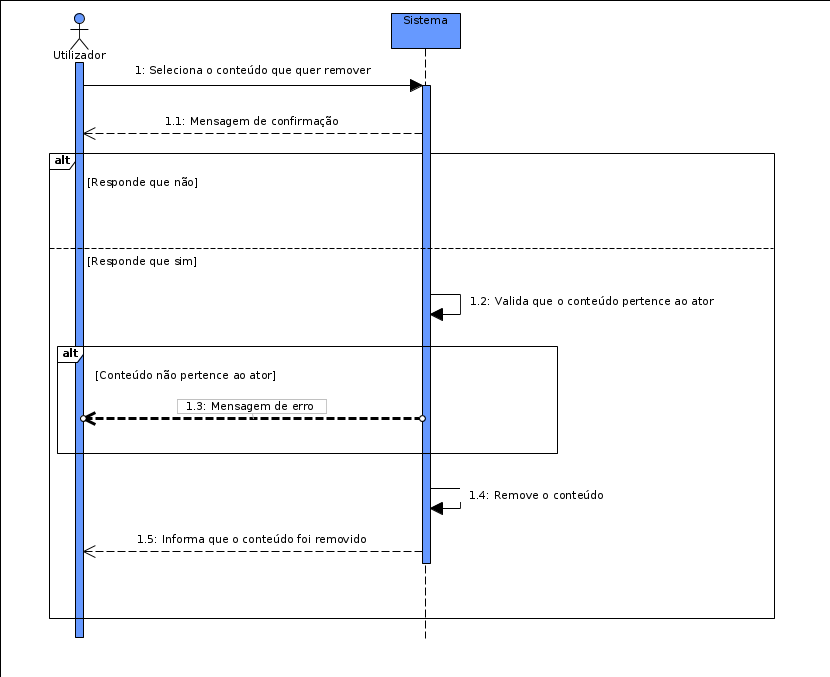
\includegraphics[width=\textwidth]{images/remconteudoSeq.png}  
    \caption{Diagrama de sequência do Remover Conteúdo}
\end{figure}

\section{Alterar Categoria}

\begin{figure}[H]
	\centering 
    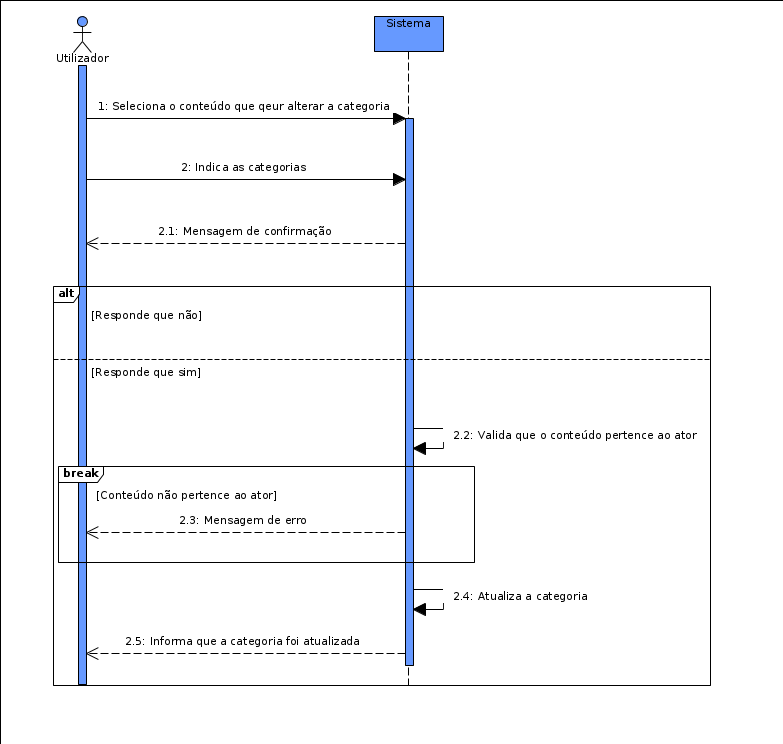
\includegraphics[width=\textwidth]{images/altcategoriaSeq.png}  
    \caption{Diagrama de sequência do Alterar Categoria}
\end{figure}

\section{Criar Playlist}

\begin{figure}[H]
	\centering 
    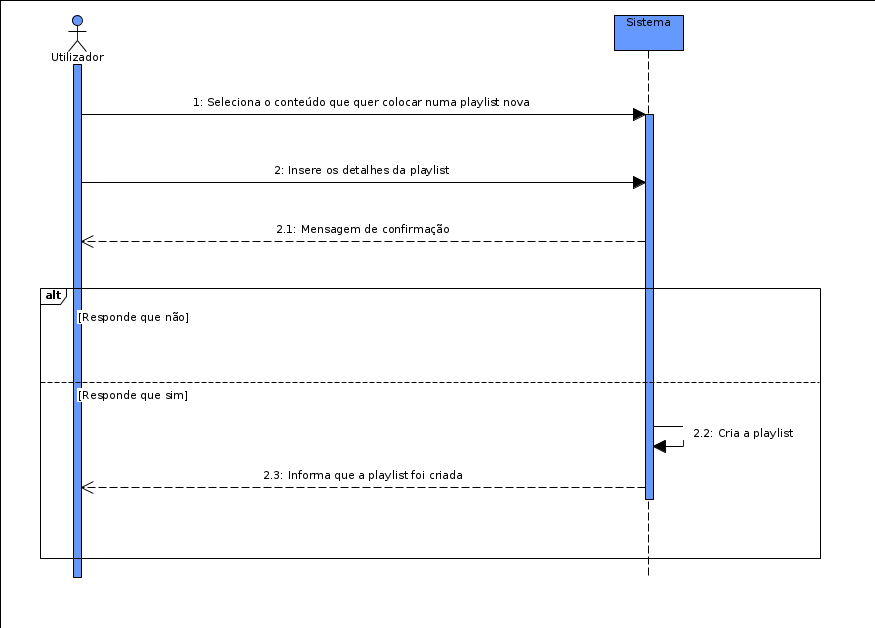
\includegraphics[width=\textwidth]{images/criarplaylistSeq.png}  
    \caption{Diagrama de sequência do Criar Playlist}
\end{figure}

\section{Remover Playlist}

\begin{figure}[H]
	\centering 
    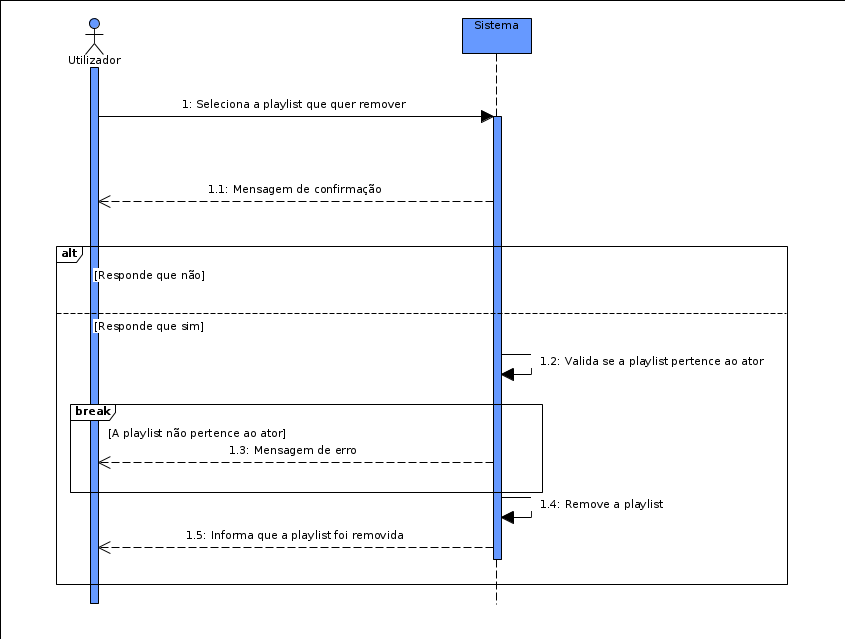
\includegraphics[width=\textwidth]{images/remplaylistSeq.png}  
    \caption{Diagrama de sequência do Remover Playlist}
\end{figure}

\section{Reproduzir Conteúdo}

\begin{figure}[H]
	\centering 
    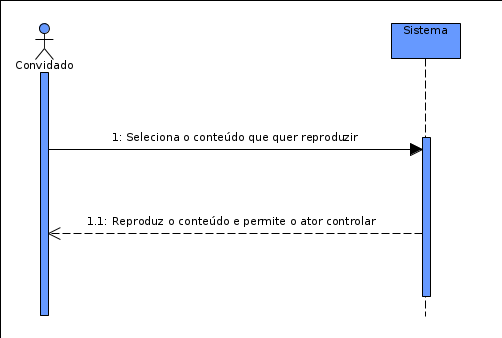
\includegraphics[width=\textwidth]{images/repconteudoSeq.png}  
    \caption{Diagrama de sequência do Reproduzir Conteúdo}
\end{figure}

\section{Registar Utilizador}

\begin{figure}[H]
	\centering 
    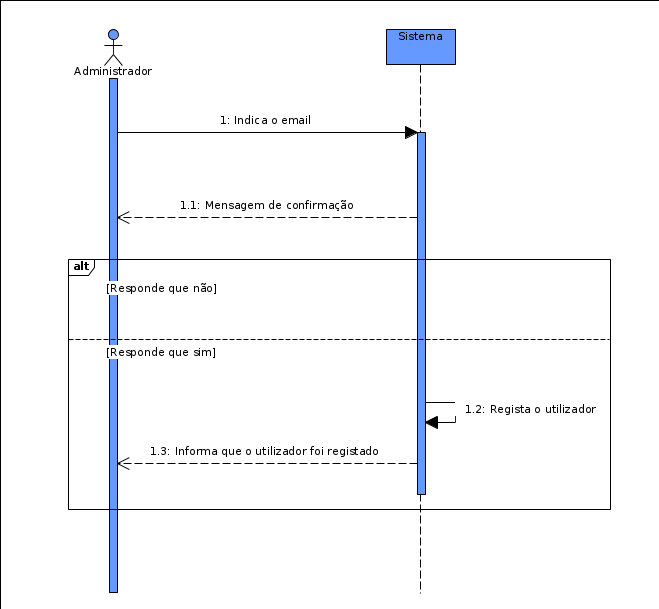
\includegraphics[width=\textwidth]{images/reguserSeq.png}  
    \caption{Diagrama de sequência do Registar Utilizador}
\end{figure}

\section{Eliminar Utilizador}

\begin{figure}[H]
	\centering 
    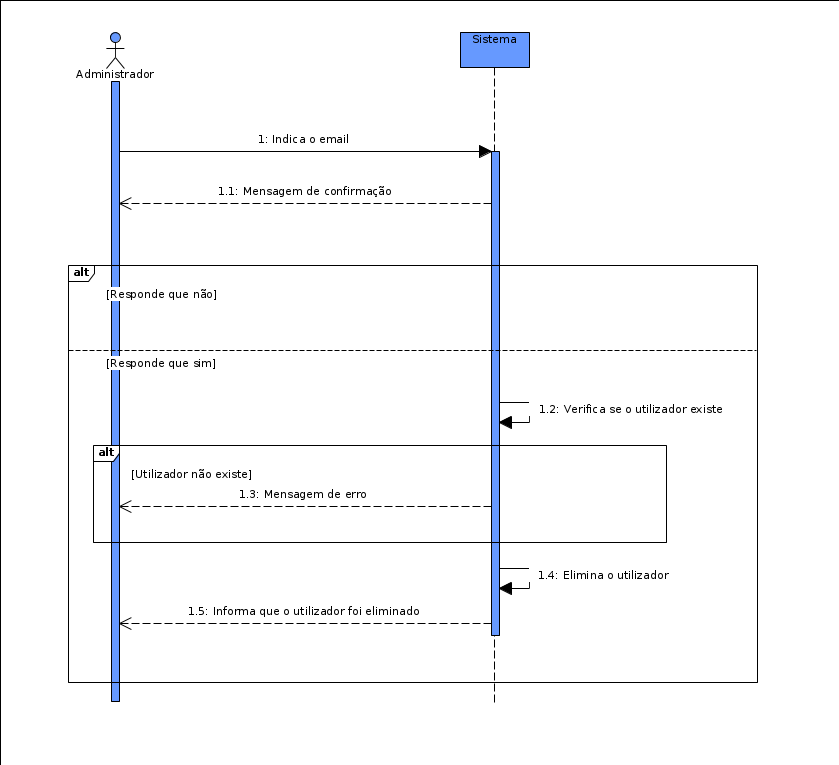
\includegraphics[width=\textwidth]{images/elemuserSeq.png}  
    \caption{Diagrama de sequência do Eliminar Utilizador}
\end{figure}

\section{Fazer Convite}

\begin{figure}[H]
	\centering 
    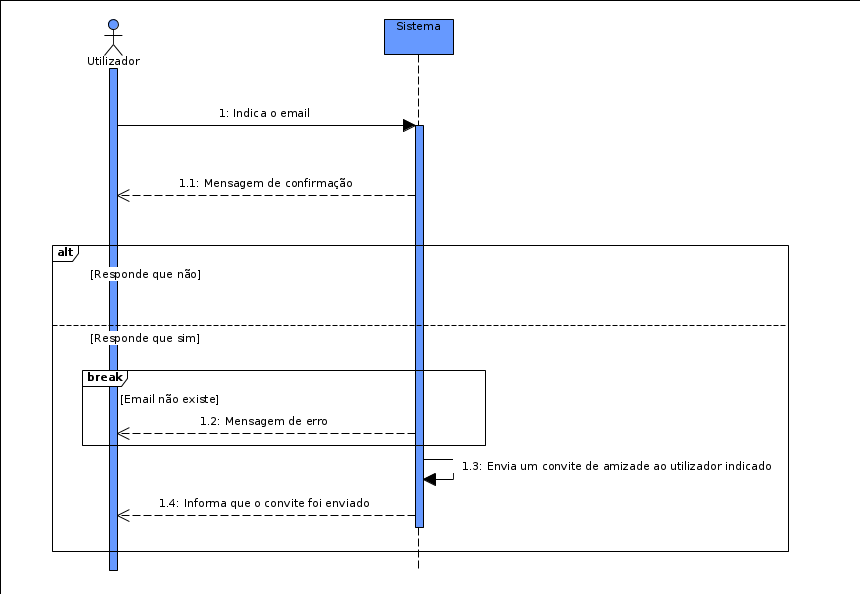
\includegraphics[width=\textwidth]{images/fazerconviteSeq.png}  
    \caption{Diagrama de sequência do Fazer Convite}
\end{figure}

\section{Responder a convite}

\begin{figure}[H]
	\centering 
    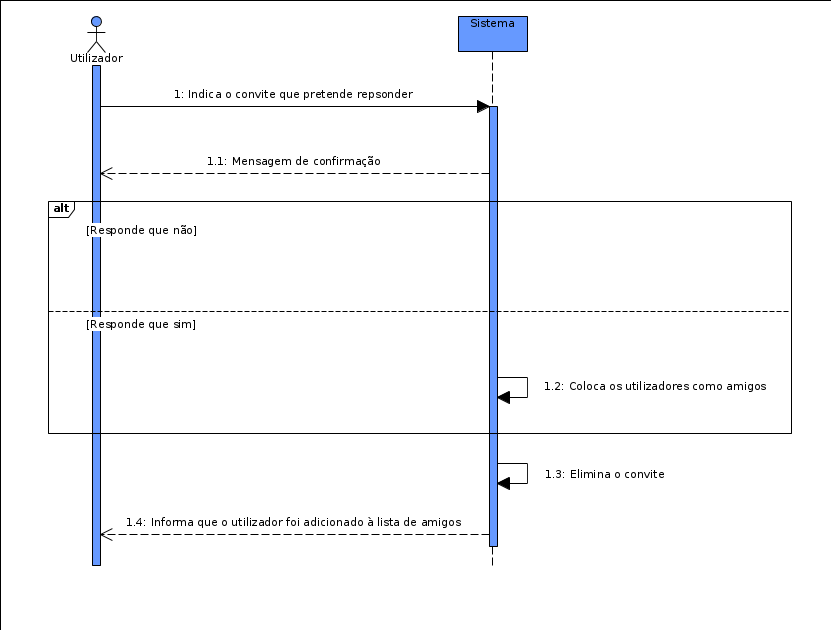
\includegraphics[width=\textwidth]{images/respconviteSeq.png}  
    \caption{Diagrama de sequência do Responder a Convite}
\end{figure}

\section{Remover Amigo}

\begin{figure}[H]
	\centering 
    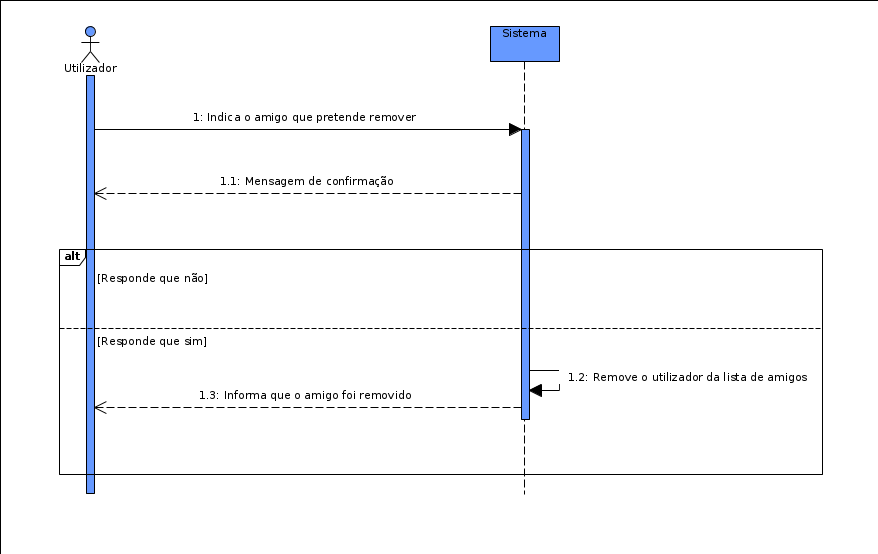
\includegraphics[width=\textwidth]{images/remamigoSeq.png}  
    \caption{Diagrama de sequência do Remover Amigo}
\end{figure}

\section{Editar Utilizador}

\begin{figure}[H]
	\centering 
    \includegraphics[width=\textwidth]{images/edituserSeq.png}  
    \caption{Diagrama de sequência do Editar Utilizador}
\end{figure}

\chapter{Diagramas de Máquina Estado}

Para uma melhor demonstração e planeamento dos estados da aplicação são criados os
diagramas de Máquina Estado. A modelação destes é muito importante pois permite
mostrar todos os estados possíveis que podem ser tomados. Para isso foram modelados
4 diagramas:

\section{Diagrama de Máquina Estado Principal - Login}

Este diagrama demonstra o primeiro passo que cada user terá que tomar antes de 
interagir com o sistema. Quando é realizado o Login o utilizador tem ou não de 
inserir as suas credenciai, podendo ser tomados estados
diferentes. O primeiro estado acontece quando o ator que está a interagir
com o sistema não possui conta mas pretende utiliza-lo, então entra como
convidado. O segundo estado acontece quando o ator possui conta e o terceiro
quando o ator que inseriu as credenciais para fazer login tem privilégios de 
administrador.

\section{Diagrama de Máquina Estado Convidado}

Um convidado pode aceder ao media presente no sistema e pode reproduzi-lo.

\section{Diagrama de Máquina Estado Utilizador}

Um utilizador é um Convidado mas com funcionalidades a mais. Além
de conseguir só reproduzir media, pode fazer upload/download do mesmo, criar
playlists e alterar as suas credenciais.

\section{Diagrama de Máquina Estado Administrador}

Um administrador é idêntico a um utilizador mas com mais duas funcionalidades:
criação e remoção de contas atráves do email.

\chapter{Diagrama de Classes}

Com base no modelo de Dominio decidimos criar as classes apresentadas na figura abaixo,
exceto uma (MediaCenter) que foi acrescida por decisão nossa para melhor manutenção
da aplicação e serve como a classe "principal" do projeto.

\begin{figure}[H]
	\centering 
    \includegraphics[width=\textwidth]{images/classdiagram.png}  
    \caption{Diagrama de Classes}
\end{figure}

\chapter{Diagrama de Packages}

Na criação dos packages tivemos em mente dois grupos: o que agrupa as classes que 
interajem com os atores do sistema e o que agrupa as classes relacionadas com o media.
Assim o manuseamento será muito mais "fácil" quando for necessário tratar de um use case
especifico.

\begin{figure}[H]
	\centering 
    \includegraphics[width=\textwidth]{images/packages.png}  
    \caption{Diagrama de Packages}
\end{figure}

\chapter{Diagramas de Sequência de Sistemas}

No capitulo anterior foi apresentado como o sistema está estruturado relativamente aos
packages, e com isso foi nos dado a oportunidade de voltar a analisar cada um
dos use cases mas desta vez com base nos subsistemas criados: Media e Users.

\section{Login}

\begin{figure}[H]
	\centering 
    \includegraphics[width=\textwidth]{images/loginSub.png}  
    \caption{Diagrama de sequência de subsistema do Login}
\end{figure}

\section{Logout}

\begin{figure}[H]
	\centering 
    \includegraphics[width=\textwidth]{images/logoutSub.png}  
    \caption{Diagrama de sequência de subsistema do Logout}
\end{figure}

\section{Entrar como convidado}

\begin{figure}[H]
	\centering 
    \includegraphics[width=\textwidth]{images/convidadoSub.png}  
    \caption{Diagrama de sequência de subsistema do Entrar como Convidado}
\end{figure}

\section{Upload}

\begin{figure}[H]
	\centering 
    \includegraphics[width=\textwidth]{images/uploadSub.png}  
    \caption{Diagrama de sequência de subsistema do Upload}
\end{figure}

\section{Download}

\begin{figure}[H]
	\centering 
    \includegraphics[width=\textwidth]{images/downloadSub.png}  
    \caption{Diagrama de sequência de subsistema do Download}
\end{figure}

\section{Remover Conteúdo}

\begin{figure}[H]
	\centering 
    \includegraphics[width=\textwidth]{images/remconteudoSub.png}  
    \caption{Diagrama de sequência de subsistema do Remover Conteúdo}
\end{figure}

\section{Alterar Categoria}

\begin{figure}[H]
	\centering 
    \includegraphics[width=\textwidth]{images/altcategoriaSub.png}  
    \caption{Diagrama de sequência de subsistema do Alterar Categoria}
\end{figure}

\section{Criar Playlist}

\begin{figure}[H]
	\centering 
    \includegraphics[width=\textwidth]{images/criarplaylistSub.png}  
    \caption{Diagrama de sequência de subsistema do Criar Playlist}
\end{figure}

\section{Remover Playlist}

\begin{figure}[H]
	\centering 
    \includegraphics[width=\textwidth]{images/remplaylistSub.png}  
    \caption{Diagrama de sequência de subsistema do Remover Playlist}
\end{figure}

\section{Reproduzir Conteúdo}

\begin{figure}[H]
	\centering 
    \includegraphics[width=\textwidth]{images/repconteudoSub.png}  
    \caption{Diagrama de sequência de subsistema do Reproduzir Conteúdo}
\end{figure}

\section{Registar Utilizador}

\begin{figure}[H]
	\centering 
    \includegraphics[width=\textwidth]{images/reguserSub.png}  
    \caption{Diagrama de sequência de subsistema do Registar Utilizador}
\end{figure}

\section{Eliminar Utilizador}

\begin{figure}[H]
	\centering 
    \includegraphics[width=\textwidth]{images/elemuserSub.png}  
    \caption{Diagrama de sequência de subsistema do Eliminar Utilizador}
\end{figure}

\section{Fazer Convite}

\begin{figure}[H]
	\centering 
    \includegraphics[width=\textwidth]{images/fazerconviteSub.png}  
    \caption{Diagrama de sequência de subsistema do Fazer Convite}
\end{figure}

\section{Responder a convite}

\begin{figure}[H]
	\centering 
    \includegraphics[width=\textwidth]{images/respconviteSub.png}  
    \caption{Diagrama de sequência de subsistema do Responder a Convite}
\end{figure}

\section{Remover Amigo}

\begin{figure}[H]
	\centering 
    \includegraphics[width=\textwidth]{images/remamigoSub.png}  
    \caption{Diagrama de sequência de subsistema do Remover Amigo}
\end{figure}

\section{Editar Utilizador}

\begin{figure}[H]
	\centering 
    \includegraphics[width=\textwidth]{images/edituserSub.png}  
    \caption{Diagrama de sequência de subsistema do Editar Utilizador}
\end{figure}

\chapter{Diagramas de Sequência de Implementação}

Com os diagramas de sequência de subsistemas modulados no capítulo anterior,
agora desenvolvemos os de implementação. Estes são mais detalhades e contém
mais informações que os anteriores pois já fazem referência às classes e
funções que serão utilizadas no código.

\section{Login}

\begin{figure}[H]
	\centering 
    \includegraphics[width=\textwidth]{images/loginImp.png}  
    \caption{Diagrama de sequência de implementação do Login}
\end{figure}

\section{Logout}

\section{Entrar como convidado}

\section{Upload}

\begin{figure}[H]
	\centering 
    \includegraphics[width=\textwidth]{images/uploadImp.png}  
    \caption{Diagrama de sequência de implementação do Upload}
\end{figure}

\section{Download}

\section{Remover Conteúdo}

\section{Alterar Categoria}

\section{Criar Playlist}

\section{Remover Playlist}

\section{Reproduzir Conteúdo}

\section{Registar Utilizador}

\begin{figure}[H]
	\centering 
    \includegraphics[width=\textwidth]{images/criarUserImp.png}  
    \caption{Diagrama de sequência de implementação do Registar Utilizador}
\end{figure}

\section{Eliminar Utilizador}

\begin{figure}[H]
	\centering 
    \includegraphics[width=\textwidth]{images/remUserImp.png}  
    \caption{Diagrama de sequência de implementação do Eliminar Utilizador}
\end{figure}

\section{Fazer Convite}

\section{Responder a convite}

\section{Remover Amigo}

\section{Editar Utilizador}

\subsection{Nome}

\begin{figure}[H]
	\centering 
    \includegraphics[width=\textwidth]{images/editUserNameImp.png}  
    \caption{Diagrama de sequência de implementação do Editar Utilizador - Nome}
\end{figure}

\subsection{Password}

\begin{figure}[H]
	\centering 
    \includegraphics[width=\textwidth]{images/editUserPassImp.png}  
    \caption{Diagrama de sequência de implementação do Editar Utilizador - Password}
\end{figure}

\chapter{Base de Dados}

De modo a deixarmos de guardar os dados em memória construímos uma base de dados
que será indispensável para o armazenamento das informações para um bom funcionamento
do nosso software.
Na figura seguinte é possível vizualizar o modelo lógico da base de dados.

\end{document}
